\documentclass[aspectratio=169]{beamer}
% ============================================================================
% HEC Montréal MBA -- ECON50803: Macroeconomic Environment
% Shared Beamer Preamble
% ============================================================================

% --- Theme and base settings ------------------------------------------------
\usetheme{default}
\setbeamersize{text margin left=1.2cm, text margin right=1.2cm}

% --- Fonts ------------------------------------------------------------------
% Sans-serif throughout for a business look (comment out FiraSans if unavailable)
\usepackage[sfdefault,light]{FiraSans}
\usepackage{FiraMono}
\usepackage[T1]{fontenc}
\usepackage[utf8]{inputenc}
\setbeamerfont{title}{series=\bfseries, size=\Large}
\setbeamerfont{frametitle}{series=\bfseries, size=\large}
\setbeamerfont{framesubtitle}{series=\mdseries, size=\normalsize}

% --- Colors -----------------------------------------------------------------
\definecolor{HECnavy}{HTML}{002855}
\definecolor{HECgreen}{HTML}{26d07c}
\definecolor{HECcoral}{HTML}{ff585d}
\definecolor{HECtext}{HTML}{2D3748}
\definecolor{HECgray}{HTML}{94A3B8}
\definecolor{HEClightgray}{HTML}{F1F5F9}
\definecolor{HEClightblue}{HTML}{E8EDF3}

% Beamer color assignments
\setbeamercolor{normal text}{fg=HECtext}
\setbeamercolor{title}{fg=HECnavy}
\setbeamercolor{frametitle}{fg=HECnavy}
\setbeamercolor{structure}{fg=HECnavy}
\setbeamercolor{background canvas}{bg=white}
\setbeamercolor{alerted text}{fg=HECcoral}
\setbeamercolor{example text}{fg=HECgreen}
\hypersetup{colorlinks, linkcolor=HECnavy, urlcolor=HECnavy, citecolor=HECtext}

% --- Navigation and chrome --------------------------------------------------
\setbeamertemplate{navigation symbols}{}

% Frame title: bold text with a thin accent line
\setbeamertemplate{frametitle}{%
   \vspace{0.25cm}%
   {\usebeamerfont{frametitle}\usebeamercolor[fg]{frametitle}\insertframetitle}%
   \ifx\insertframesubtitle\empty\else%
      \\[2pt]{\usebeamerfont{framesubtitle}\textcolor{HECgray}{\insertframesubtitle}}%
   \fi%
   \\[-4pt]\textcolor{HECgreen}{\rule{2.5cm}{1.5pt}}%
   \\[-2pt]%
}

% Footer: course name left, slide number right, thin rule above
\setbeamertemplate{footline}{%
   \vspace{-0.1cm}%
   \hbox to \paperwidth{%
      \hspace{1.2cm}%
      \textcolor{HEClightgray}{\rule{0.84\paperwidth}{0.4pt}}%
      \hspace{1.2cm}%
   }%
   \vspace{0.05cm}%
   \hbox to \paperwidth{%
      \hspace{1.2cm}%
      {\scriptsize\textcolor{HECgray}{ECON 50803\enspace\textbar\enspace Environnement macroéconomique}}%
      \hfill%
      {\scriptsize\textcolor{HECgray}{\insertframenumber}}%
      \hspace{1.2cm}%
   }%
   \vspace{0.15cm}%
}

% --- Itemize/enumerate styling ----------------------------------------------
\setbeamertemplate{itemize item}{\textcolor{HECnavy}{$\bullet$}}
\setbeamertemplate{itemize subitem}{\textcolor{HECgray}{$\bullet$}}
\setbeamertemplate{itemize subsubitem}{\textcolor{HECgray}{\scalebox{0.6}{$\blacktriangleright$}}}
\setbeamertemplate{enumerate item}{\textcolor{HECnavy}{\bfseries\insertenumlabel.}}
\setbeamertemplate{enumerate subitem}{\textcolor{HECgray}{\insertsubenumlabel.}}

% --- Packages ---------------------------------------------------------------
\usepackage{
   tikz, caption, subcaption, ragged2e, amsmath, bm,
   makecell, threeparttable, booktabs, mathtools,
   multirow, calc, hyperref, tabularx, colortbl,
   transparent, tcolorbox, xcolor, graphicx
}
\usepackage[round]{natbib}
\usetikzlibrary{decorations.pathreplacing, decorations.markings, calc, arrows.meta, positioning}
\usepackage[absolute,overlay]{textpos}
\captionsetup[figure]{labelformat=empty, font=small, textfont=it}
\captionsetup[table]{labelformat=empty, font=small}
\setlength{\belowcaptionskip}{0cm}
\apptocmd{\frame}{}{\justifying}

% --- Paths ------------------------------------------------------------------
\graphicspath{{../Figures/}}
\newcommand*\includetables[1]{\input{../Tables/#1.tex}}

% --- Mathematical commands --------------------------------------------------
\DeclareMathOperator*{\argmax}{arg\,max}
\newcommand{\partialof}[2]{\frac{\partial #1}{\partial #2}}
\newcommand{\totalof}[2]{\frac{\text{d}#1}{\text{d}#2}}
\newcommand{\pctchg}[1]{\%\Delta #1}
\newcommand{\smallquad}{\hspace{0.5em}}

% --- Resize equation command ------------------------------------------------
\newcommand{\resizeeq}[2]{\resizebox{#2\hsize}{!}{$#1$}}

% ============================================================================
% CUSTOM SLIDE TYPES
% ============================================================================

% --- Title slide (call with \titleframe) ------------------------------------
\newcommand{\titleframe}{%
   {\setbeamertemplate{footline}{}%
   \begin{frame}[plain]
      \begin{tikzpicture}[remember picture, overlay]
         % Navy accent bar on the left
         \fill[HECnavy] (current page.north west) rectangle
            ([xshift=0.6cm]current page.south west);
         % Green accent line
         \fill[HECgreen] ([xshift=0.6cm]current page.north west) rectangle
            ([xshift=0.65cm]current page.south west);
      \end{tikzpicture}
      \vspace{1cm}
      \hspace{0.6cm}%
      \begin{minipage}{0.85\textwidth}
         {\usebeamerfont{title}\usebeamercolor[fg]{title}\inserttitle}
         \\[12pt]
         \textcolor{HECgreen}{\rule{3cm}{2pt}}
         \\[12pt]
         {\large\textcolor{HECgray}{\insertauthor}}
         \\[6pt]
         {\normalsize\textcolor{HECgray}{\insertdate}}
      \end{minipage}
      \vfill
      \hspace{0.6cm}%
      {\footnotesize\textcolor{HECgray}{HEC Montréal \enspace\textbar\enspace MBA}}
      \vspace{0.5cm}
   \end{frame}}%
}

% --- Section divider slide --------------------------------------------------
\newcommand{\sectionframe}[1]{%
   {\setbeamertemplate{footline}{}%
   \begin{frame}[plain]
      \begin{tikzpicture}[remember picture, overlay]
         \fill[HECnavy] ([shift={(-1pt,1pt)}]current page.north west) rectangle
            ([shift={(1pt,-1pt)}]current page.south east);
         \node[anchor=center] at (current page.center) {%
            \begin{minipage}{0.8\paperwidth}
               \centering
               {\LARGE\bfseries\textcolor{white}{#1}}
               \\[12pt]
               \textcolor{HECgreen}{\rule{3cm}{2pt}}
            \end{minipage}
         };
      \end{tikzpicture}
   \end{frame}}%
}

% ============================================================================
% CUSTOM BOX ENVIRONMENTS
% ============================================================================

% Key Insight (green accent)
\newtcolorbox{keyinsight}[1][Point clé]{%
   colback=HECgreen!5,
   colframe=HECgreen,
   boxrule=0pt,
   leftrule=3pt,
   arc=8pt,
   title={\textcolor{HECgreen}{\bfseries #1}},
   coltitle=HECgreen,
   fonttitle=\bfseries,
   attach title to upper={\\[4pt]},
   left=10pt, right=10pt, top=6pt, bottom=6pt
}

% Business Implication (navy accent)
\newtcolorbox{bizimplication}[1][Implication d'affaires]{%
   colback=HECnavy!5,
   colframe=HECnavy,
   boxrule=0pt,
   leftrule=3pt,
   arc=8pt,
   title={\textcolor{HECnavy}{\bfseries #1}},
   coltitle=HECnavy,
   fonttitle=\bfseries,
   attach title to upper={\\[4pt]},
   left=10pt, right=10pt, top=6pt, bottom=6pt
}

% Warning / Important (coral accent)
\newtcolorbox{warning}[1][Important]{%
   colback=HECcoral!5,
   colframe=HECcoral,
   boxrule=0pt,
   leftrule=3pt,
   arc=8pt,
   title={\textcolor{HECcoral}{\bfseries #1}},
   coltitle=HECcoral,
   fonttitle=\bfseries,
   attach title to upper={\\[4pt]},
   left=10pt, right=10pt, top=6pt, bottom=6pt
}

% Definition (gray background)
\newtcolorbox{defbox}[1][Définition]{%
   colback=HEClightgray,
   colframe=HEClightgray,
   boxrule=0pt,
   leftrule=3pt,
   arc=8pt,
   left=10pt, right=10pt, top=6pt, bottom=6pt,
   title={\textcolor{HECnavy}{\bfseries #1}},
   coltitle=HECnavy,
   fonttitle=\bfseries,
   attach title to upper={\\[4pt]}
}

% In-Class Exercise (coral accent)
\newtcolorbox{exercise}[1][Exercice]{%
   colback=HECcoral!5,
   colframe=HECcoral,
   boxrule=0pt,
   leftrule=3pt,
   arc=8pt,
   title={\textcolor{HECcoral}{\bfseries #1}},
   coltitle=HECcoral,
   fonttitle=\bfseries,
   attach title to upper={\\[4pt]},
   left=10pt, right=10pt, top=6pt, bottom=6pt
}

% ============================================================================
% NEWSPAPER HEADLINES SLIDE TEMPLATE
% ============================================================================
% Usage: inside a frame, open a tikzpicture[remember picture, overlay], then:
%   \setcounter{newshl}{0}
%   \newsheadline{Newspaper Name}{``Headline text''}   % up to 6 entries
%   \headlinesoverlay{Large overlay text}               % optional 2nd slide
%
% Headlines are auto-positioned in a 2×3 staggered grid (left/right alternating).
%
% Logo support: place PNG files in Figures/logos/ (e.g., ft.png, economist.png).
% Use the optional argument to specify the logo file (without extension):
%   \newsheadline[ft]{Financial Times}{Headline text}   % logo + bold headline
%   \newsheadline{The Economist}{``Headline text''}      % text-only fallback

\newcounter{newshl}

\newcommand{\newsheadline}[3][]{%
   % #1 = optional logo file key (e.g., ft → logos/ft.png)
   % #2 = newspaper name (text fallback when no logo)
   % #3 = headline text
   \stepcounter{newshl}%
   \pgfmathsetmacro{\hlrow}{int((\thenewshl-1)/2)}%
   \pgfmathsetmacro{\hlcol}{int(mod(\thenewshl-1,2))}%
   \pgfmathsetmacro{\hlx}{0.8 + \hlcol * 7.8}%
   \pgfmathsetmacro{\hly}{-1.5 - \hlrow * 2.0}%
   \node[anchor=north west]
      at ([shift={(\hlx cm,\hly cm)}]current page.north west) {%
      \ifx\\#1\\%
         \begin{minipage}[t]{5.8cm}%
            \textbf{\textcolor{HECgray}{\footnotesize\MakeUppercase{#2}}}%
            \\[-1pt]%
            {\small\itshape #3}%
         \end{minipage}%
      \else%
         \begin{minipage}[c]{1.2cm}%
            \includegraphics[height=1.2cm]{logos/#1}%
         \end{minipage}%
         \hspace{6pt}%
         \begin{minipage}[c][1.2cm][c]{4.3cm}%
            \raggedright{\small\textcolor{HECtext!75}{#3}}%
         \end{minipage}%
      \fi%
   };%
}

\newcommand{\headlinesoverlay}[1]{%
   \only<2>{%
      \fill[white, opacity=0.85]
         (current page.south west) rectangle (current page.north east);%
      \node[anchor=center] at ([yshift=-0.5cm]current page.center) {%
         {\fontsize{36}{44}\selectfont\bfseries\textcolor{HECnavy}{#1}}%
      };%
   }%
}

% ============================================================================
% NAVIGATION BUTTONS (optional, for bottom-of-slide section nav)
% ============================================================================

\newlength{\buttonwidth}
\newlength{\currentxpos}
\setlength{\currentxpos}{1.2cm}
\newlength{\buttonsep}
\setlength{\buttonsep}{0.05cm}

\newcommand{\mybutton}[2]{%
   \settowidth{\buttonwidth}{#1}%
   \begin{textblock*}{\buttonwidth + 2ex}(\currentxpos, \paperheight - 2.5em)
      \hyperlink{#2}{\beamerbutton{#1}}
   \end{textblock*}%
   \addtolength{\currentxpos}{\buttonwidth + \buttonsep}%
}

% ============================================================================
% BACKUP SLIDES SUPPORT
% ============================================================================

\newcommand{\backupbegin}{%
   \newcounter{finalframe}%
   \setcounter{finalframe}{\value{framenumber}}%
}
\newcommand{\backupend}{%
   \setcounter{framenumber}{\value{finalframe}}%
}


\title{Cycles économiques}
\author{Jean-Félix Brouillette}
\date{Séance 4}

\begin{document}

% ============================================================================
\titleframe
% ============================================================================

{
\setbeamertemplate{footline}{}
\begin{frame}{Le macroéconomie de court terme}
   \begin{tikzpicture}[remember picture, overlay]
      \setcounter{newshl}{0}
      \newsheadline[economist]{The Economist}{\guillemotleft~The nightmare Iran energy scenario is becoming reality~\guillemotright}
      \newsheadline[bloomberg]{Bloomberg}{\guillemotleft~Iran War, Oil Price Surge Put Global Economic Recovery at Risk~\guillemotright}
      \newsheadline[lapresse]{La Presse}{\guillemotleft~Contraction surprise de l'économie canadienne~\guillemotright}
      \newsheadline[ft]{Financial Times}{\guillemotleft~Scott Bessent says 15\% global tariff `likely' to be imposed this week~\guillemotright}
      \newsheadline[radiocanada]{Radio-Canada}{\guillemotleft~L'économie s'est contractée au quatrième trimestre, selon Statistique Canada~\guillemotright}
      \newsheadline[reuters]{Reuters}{\guillemotleft~Investors brace for energy shock, inflation fears from prolonged Iran conflict~\guillemotright}
   \end{tikzpicture}
\end{frame}
}

\begin{frame}{Plan}
   \begin{enumerate}
      \setlength\itemsep{0.5cm}
      \item \textbf{Faits saillants sur les cycles économiques}
      \item Tendance et fluctuations
      \item Le modèle AD-AS
      \item Anatomie d'une récession
   \end{enumerate}
\end{frame}

% ============================================================================
\sectionframe{Faits saillants sur les cycles économiques}
% ============================================================================

\begin{frame}{Que sont les cycles économiques?}
   \centering
   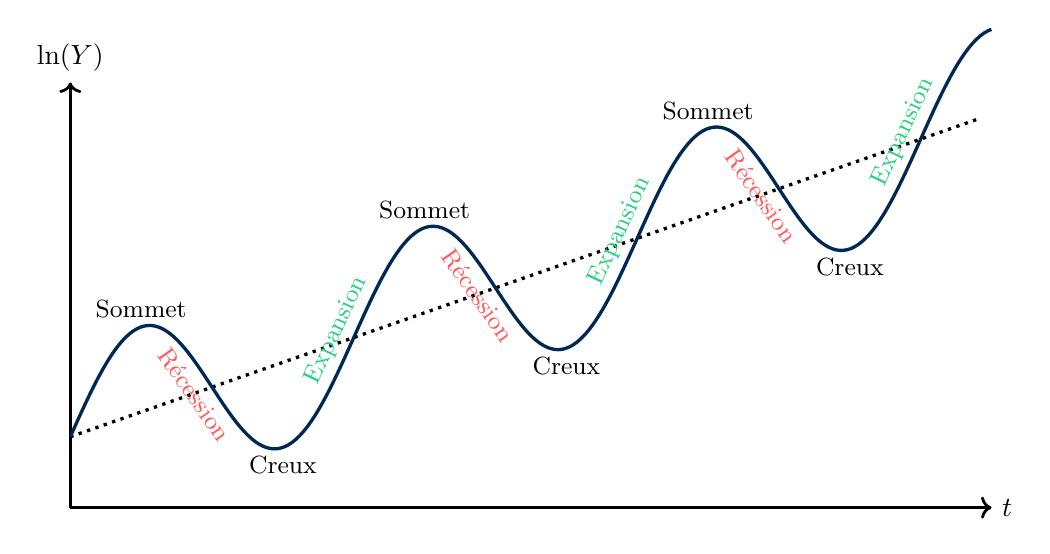
\begin{tikzpicture}[xscale=0.9, yscale=0.9,
      peak/.style={font=\small},
      trough/.style={font=\small},
      phaseE/.style={font=\small, rotate=65, HECgreen},
      phaseR/.style={font=\small, rotate=305, HECcoral}]

      % Draw the axes
      \draw[->, line width=1pt] (0,0) -- (0,6) node[above]{$\ln(Y)$};
      \draw[->, line width=1pt] (0,0) -- (13,0) node[right]{$t$};

      % Trend line: y = m x + b
      \def\slope{0.35}    % m
      \def\intercept{1}   % b
      \draw[dotted, very thick] (0,\intercept) -- (12.8,{\slope*12.8+\intercept});

      % Cyclical component: A * sin(ω x)
      \def\amp{1.2}       % amplitude (A)
      \def\omega{90}      % ω in degrees (period = 4 units)

      % Combined path:  y(x) = trend + amp * sin(ω x)
      \draw[HECnavy, very thick, samples=250, domain=0:13] plot (\x,{\slope*\x+\intercept + \amp*sin(\omega*\x)});

      % Identify the peaks and troughs
      \node[peak] at (1, {\slope*1 + \intercept + \amp + 0.25}) {Sommet};
      \node[trough] at (3, {\slope*3 + \intercept - \amp - 0.25}) {Creux};
      \node[peak] at (5, {\slope*5 + \intercept + \amp + 0.25}) {Sommet};
      \node[trough] at (7, {\slope*7 + \intercept - \amp - 0.25}) {Creux};
      \node[peak] at (9, {\slope*9 + \intercept + \amp + 0.25}) {Sommet};
      \node[trough] at (11, {\slope*11 + \intercept - \amp - 0.25}) {Creux};

      % Identify the phases
      \node[phaseR] at (1.75, {\slope*2 + \intercept - 0.1}) {Récession};
      \node[phaseE] at (3.75, {\slope*4+\intercept + 0.1}) {Expansion};
      \node[phaseR] at (5.75, {\slope*6 + \intercept - 0.1}) {Récession};
      \node[phaseE] at (7.75, {\slope*8+\intercept + 0.1}) {Expansion};
      \node[phaseR] at (9.75, {\slope*10 + \intercept - 0.1}) {Récession};
      \node[phaseE] at (11.75, {\slope*12+\intercept + 0.1}) {Expansion};
   \end{tikzpicture}
\end{frame}

\begin{frame}[t]{Expansions et récessions}
   \small
   \textbf{Expansion :} hausse du PIB réel et de l'emploi, baisse du chômage\\ \vspace{0.3cm}
   \textbf{Récession :} baisse du PIB réel et de l'emploi, hausse du chômage
   \vspace{0.2cm}
   \begin{itemize}
      \setlength\itemsep{0.2cm}
      \item \textbf{Canada :} deux trimestres consécutifs de croissance négative du PIB réel
      \item \textbf{États-Unis (NBER) :} \guillemotleft~\textit{un déclin significatif de l’activité économique étendu à l’ensemble du marché, durant plus de quelques mois, normalement visible dans le PIB réel, le revenu réel, l’emploi, la production industrielle, et les ventes de gros/détail}~\guillemotright
   \end{itemize}

   \vspace{0.1cm}
   \begin{keyinsight}[Le saviez-vous?]
      L'économie est en expansion $\sim$85\,\% du temps et en récession $\sim$15\,\% du temps.
   \end{keyinsight}
\end{frame}

\begin{frame}[t]{Cyclicité}
   \vspace{0.25cm}
   \begin{itemize}
      \setlength\itemsep{0.75cm}
      \item[] \textbf{Procyclique :} augmente en expansion, diminue en récession
         \begin{itemize}
            \item[\textcolor{HECgray}{$\bullet$}] {\small\textcolor{HECgray}{Croissance du PIB réel, consommation, investissement, emploi}}
         \end{itemize}
      \item[] \textbf{Contracyclique :} diminue en expansion, augmente en récession
         \begin{itemize}
            \item[\textcolor{HECgray}{$\bullet$}] {\small\textcolor{HECgray}{Taux de chômage, déficit budgétaire}}
         \end{itemize}
      \item[] \textbf{Acyclique :} pas de relation claire avec le cycle
         \begin{itemize}
            \item[\textcolor{HECgray}{$\bullet$}] {\small\textcolor{HECgray}{Taux d'intérêt réel, inflation}}
         \end{itemize}
   \end{itemize}
\end{frame}

\begin{frame}{Quatre faits sur les cycles économiques}
   \begin{enumerate}
      \setlength\itemsep{0.6cm}
      \item \textbf{L'investissement est plus volatil que la production et la consommation}
      \item \textbf{Les prix et les salaires sont rigides à court terme}
      \item \textbf{Il existe une faible corrélation négative entre l'inflation et le chômage}
      \item \textbf{Une courbe de rendement inversée prédit les récessions}
   \end{enumerate}
\end{frame}

\begin{frame}{L'investissement est plus volatil}
   \begin{figure}
      \centering
      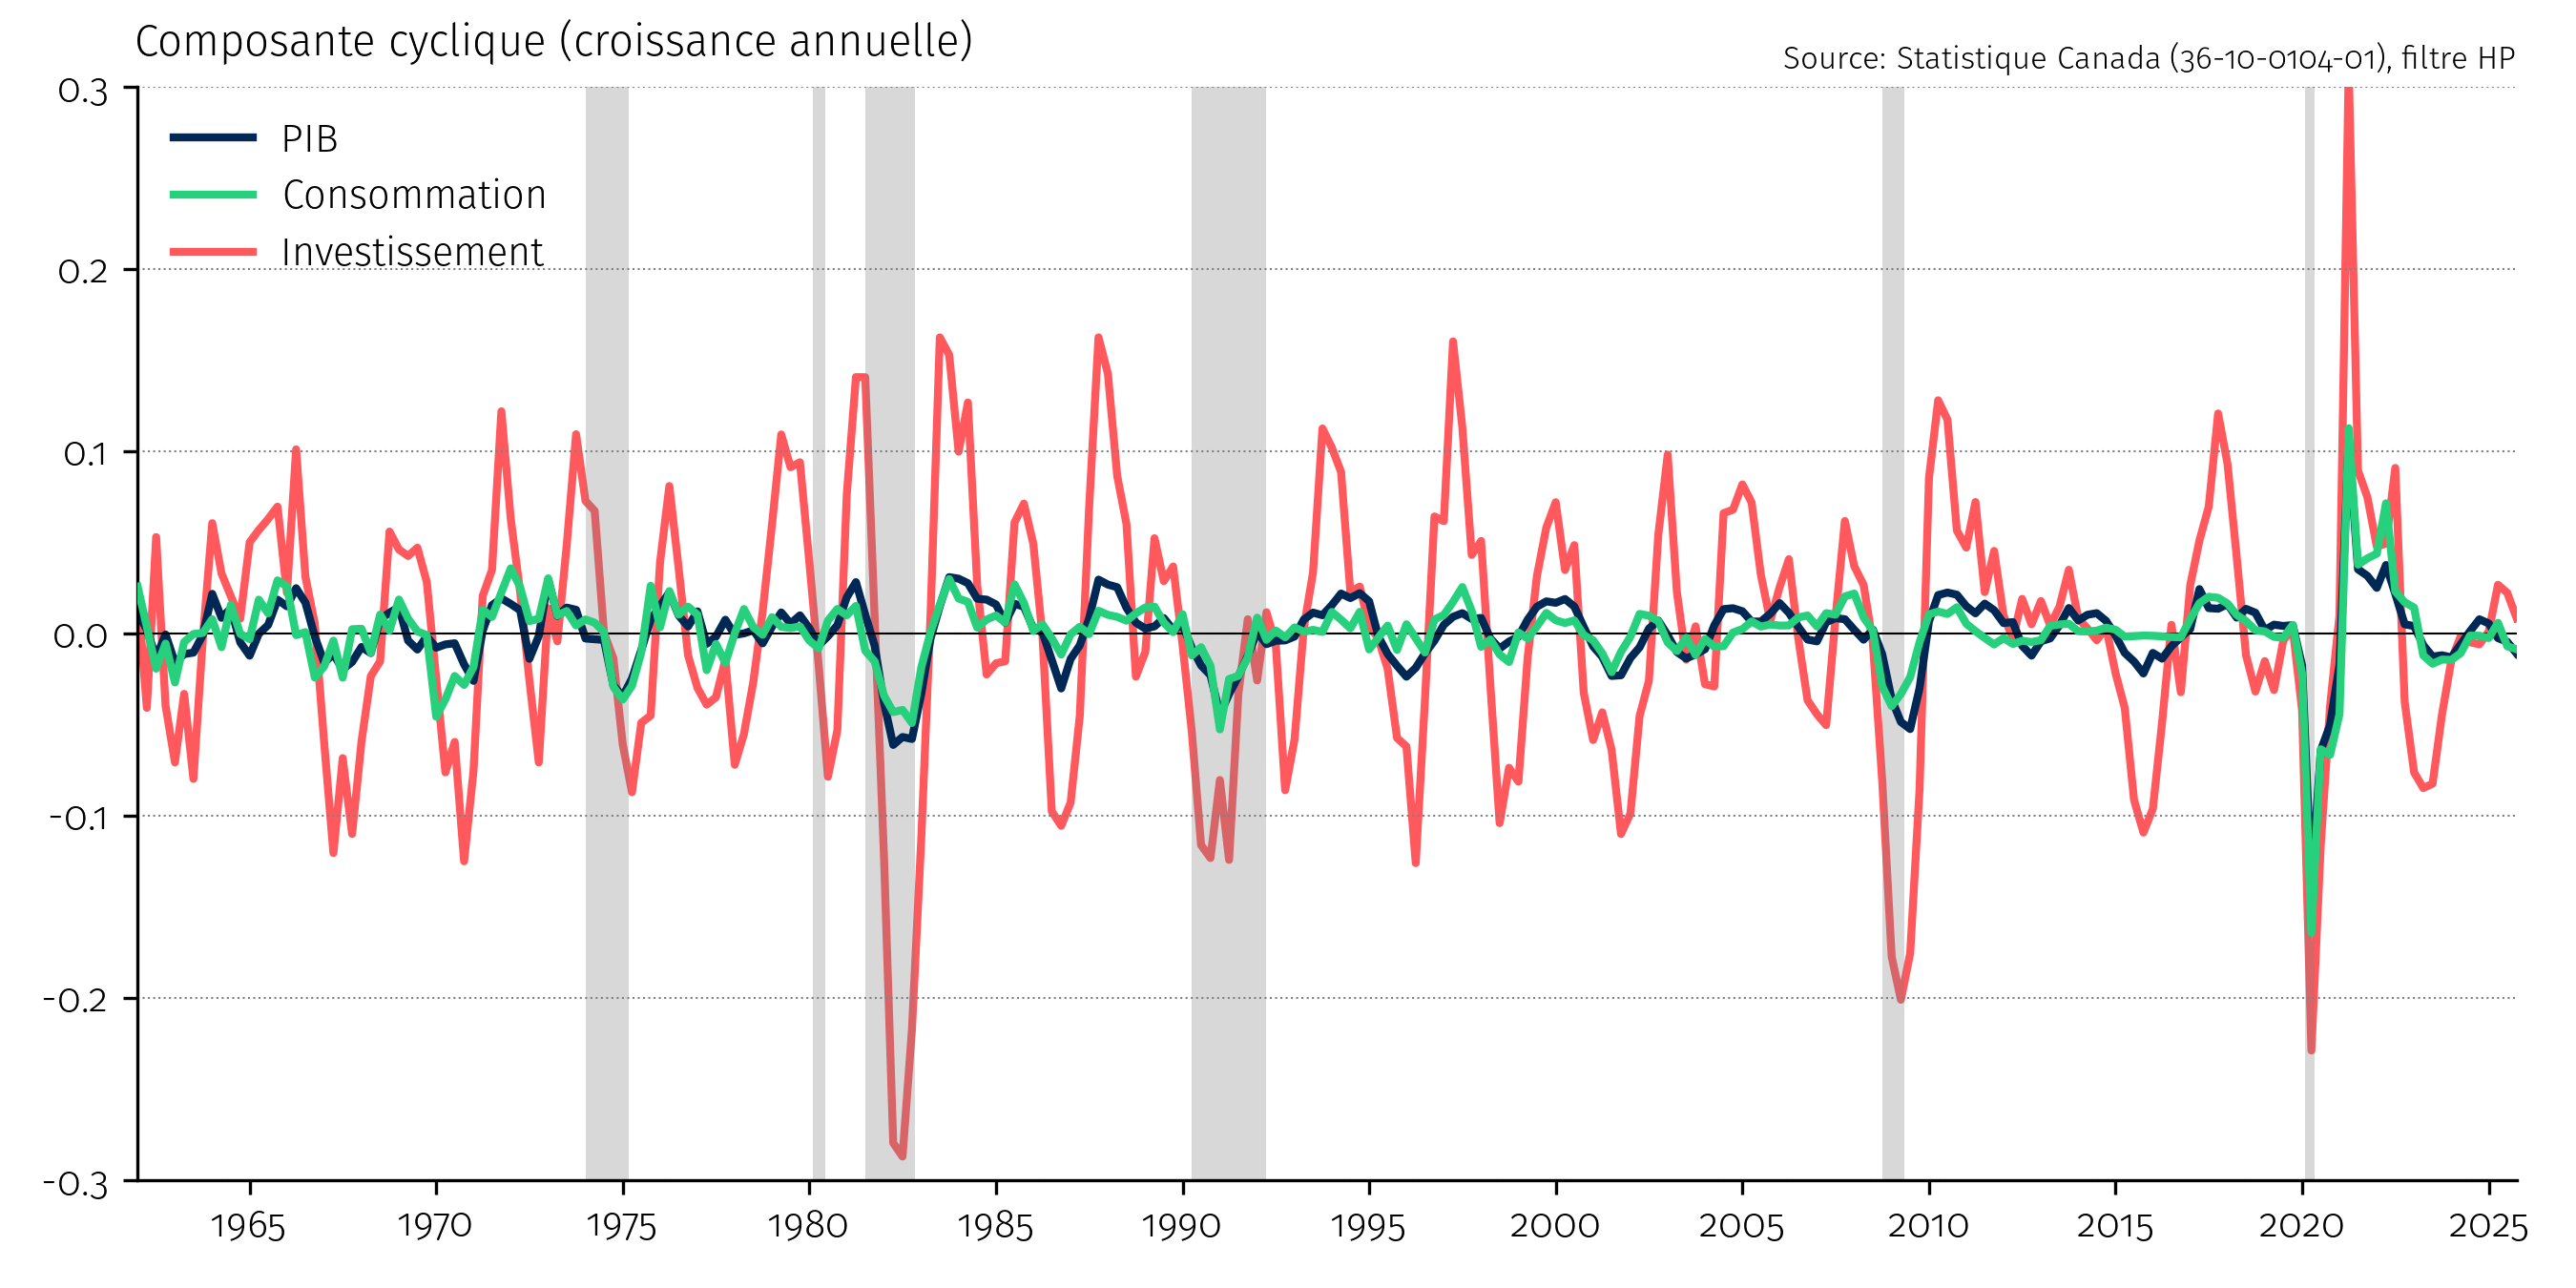
\includegraphics[width=0.95\textwidth, keepaspectratio]{cyclical_components_canada.png}
   \end{figure}
\end{frame}

\begin{frame}[t]{Les prix et les salaires sont rigides}
   \textbf{Au niveau micro :}
   \vspace{0.15cm}
   \begin{itemize}
      \setlength\itemsep{0.15cm}
      \item Durée moyenne d'un prix $\approx$ 8 mois
      \item Probabilité qu'un prix change : 11--15\,\% par mois
      \item Les salaires changent $\sim$1 fois par an
      \item Baisses de salaires très rares
      \item Les biens à forte intensité de main-d'\oe uvre ont les prix les plus rigides
   \end{itemize}
   \vspace{0.4cm}
   \textbf{Au niveau macro :}
   \vspace{0.15cm}
   \begin{itemize}
      \setlength\itemsep{0.15cm}
      \item L'inflation ne réagit pleinement aux chocs qu'après 2--3 ans
      \item Plus difficile à mesurer\ldots
   \end{itemize}
\end{frame}

\begin{frame}{La courbe de Phillips}
   \begin{figure}
      \centering
      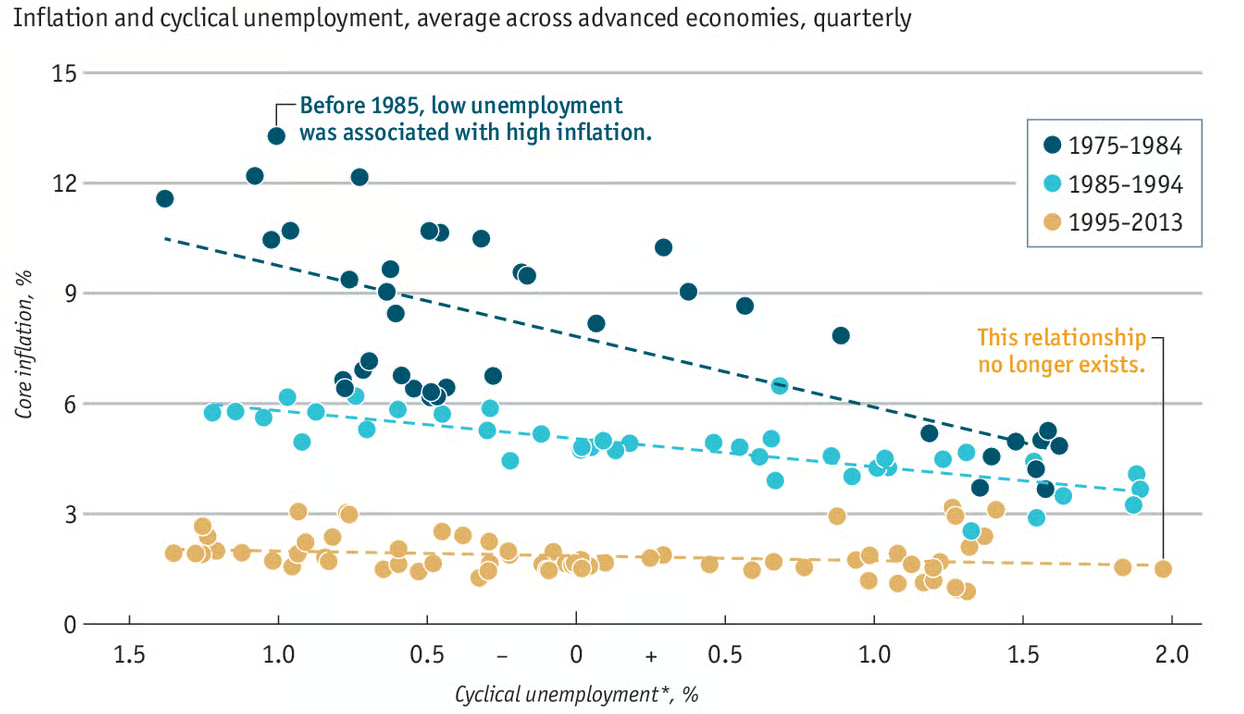
\includegraphics[width=0.85\textwidth, keepaspectratio]{phillips_curve_advanced.png}
   \end{figure}
\end{frame}

\begin{frame}[t]{La courbe de rendement inversée}
   \small
   \textbf{Normalement :} taux longs $>$ taux courts (compensation pour le risque et l'attente).

   \vspace{0.25cm}
   \textbf{Inversion :} taux courts $>$ taux longs $\to$ anticipations de \textbf{baisses de taux} futures.

   \vspace{0.25cm}
   \begin{defbox}[L'hypothèse des anticipations]
      \vspace{-0.2cm}
      \begin{equation*}
         i_{10} \approx \frac{i_{t,1} + i_{t+1,1} + \ldots + i_{t+9,1}}{10}
      \end{equation*}
      \vspace{-0.3cm}
      Si les marchés anticipent des baisses $\to$ $i_{10} < i_{1}$ $\to$ inversion.
   \end{defbox}

   \vspace{0.25cm}
   \begin{bizimplication}[Signal pour les décideurs]
      \footnotesize
      Chaque récession depuis 1970 a été précédée d'une inversion de la courbe de rendement.
   \end{bizimplication}
\end{frame}

\begin{frame}{La courbe de rendement inversée}
   \begin{figure}
      \centering
      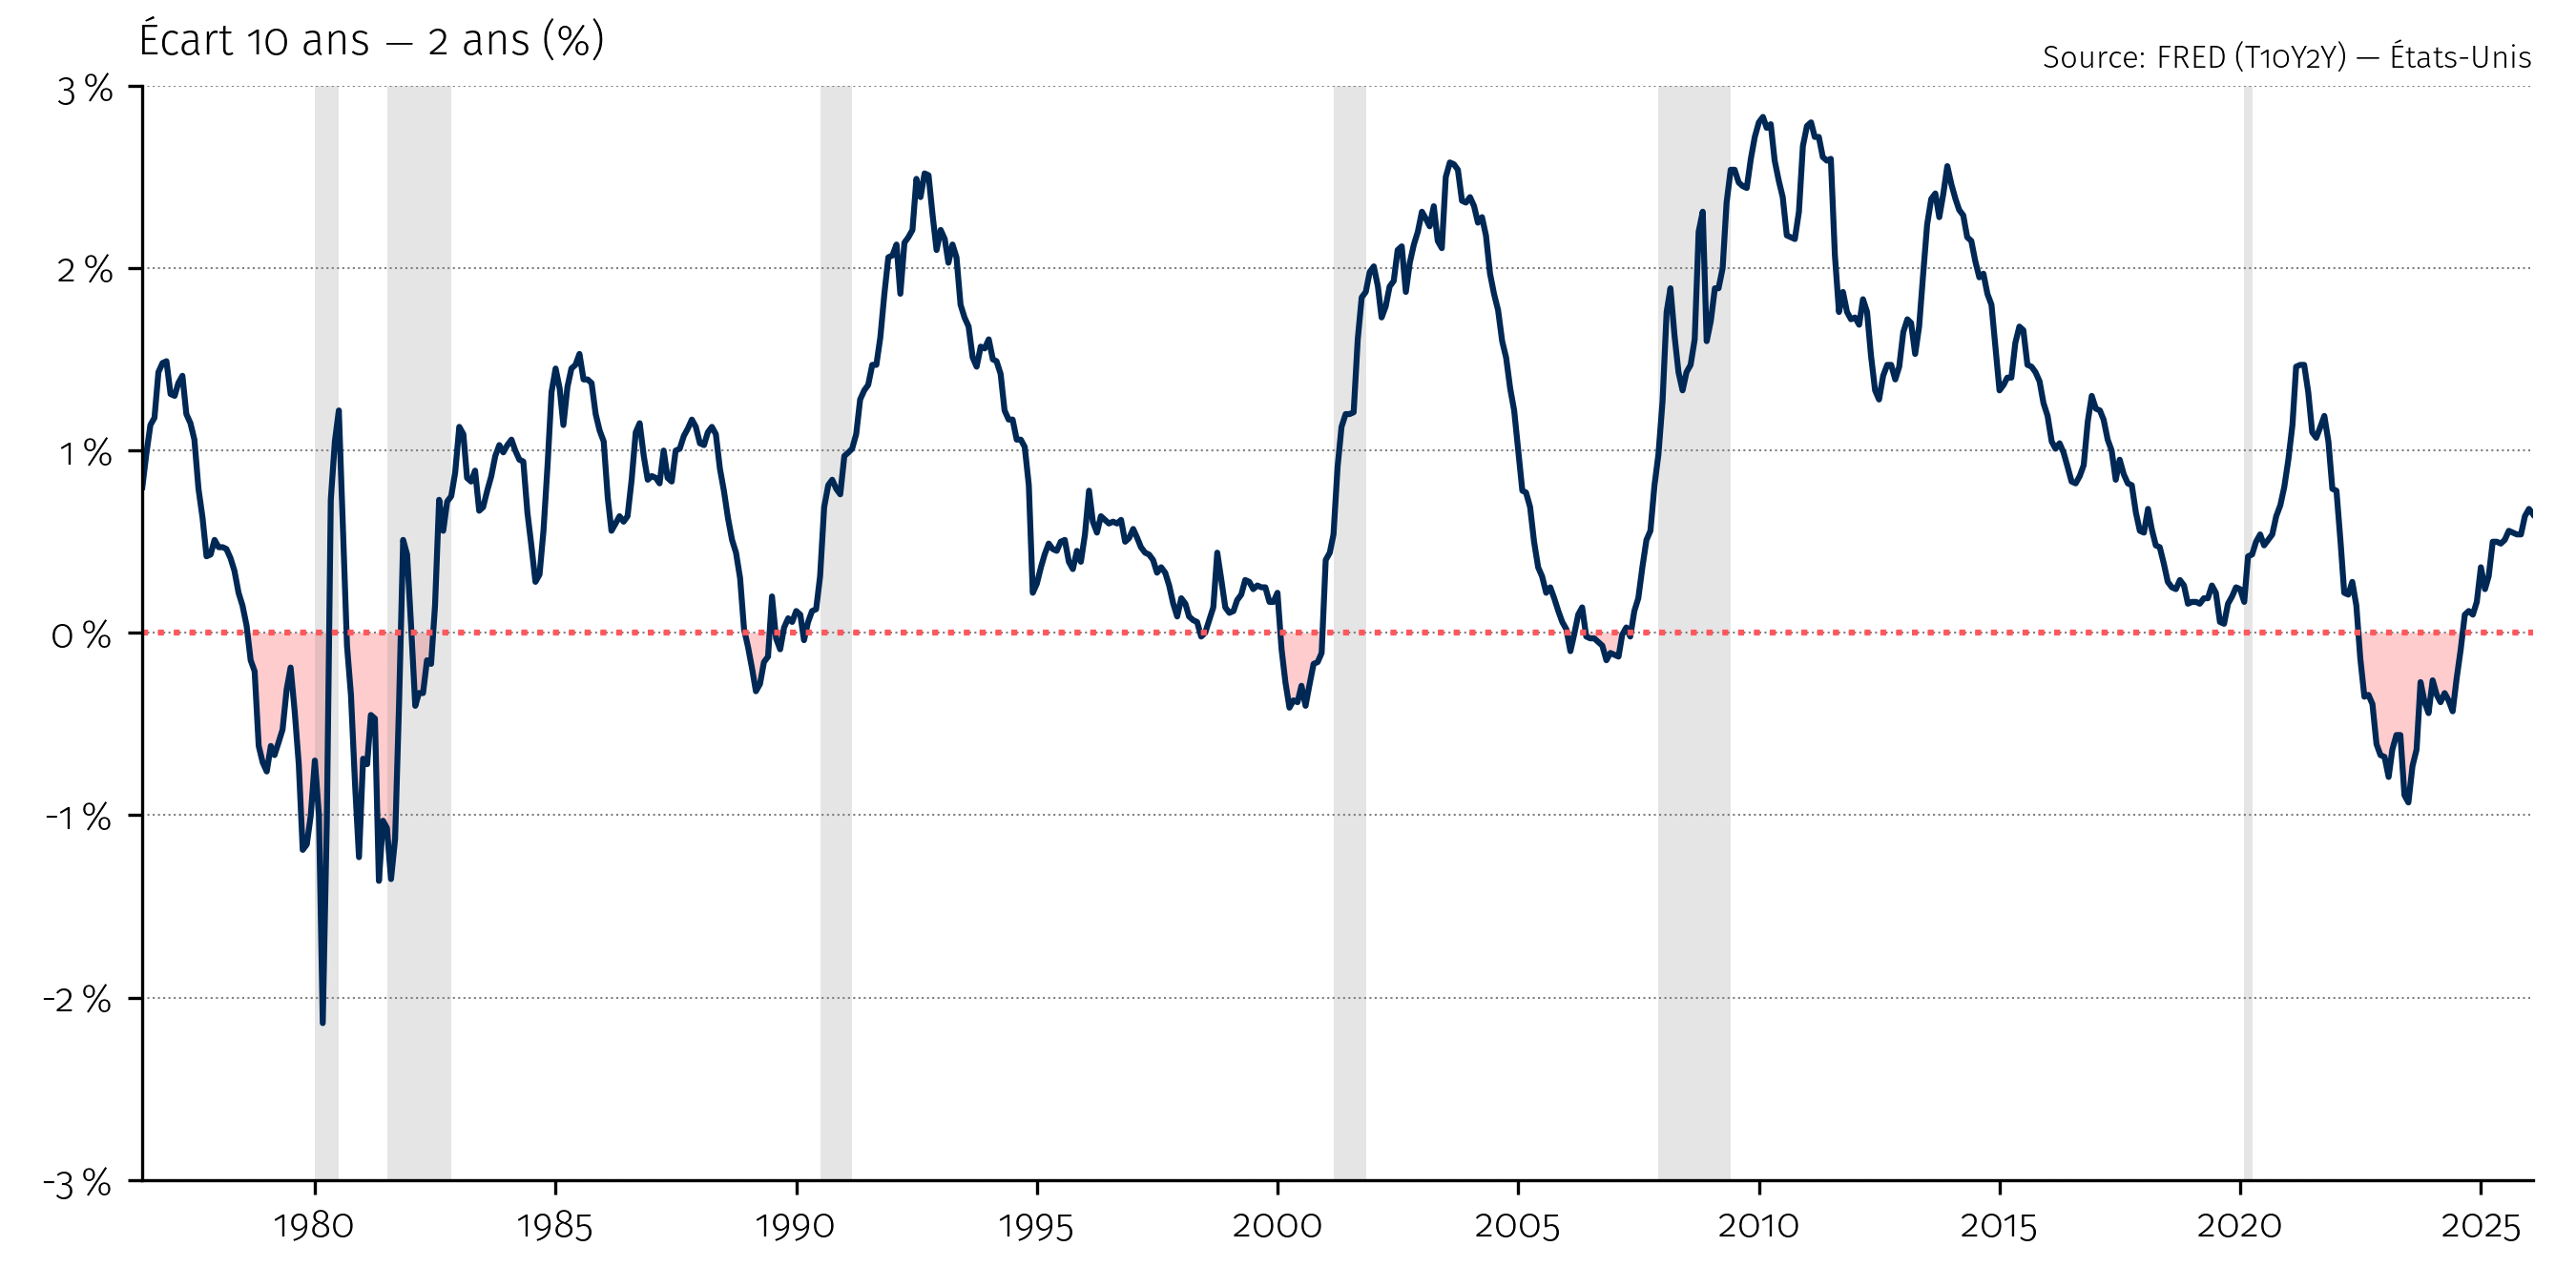
\includegraphics[width=0.95\textwidth, keepaspectratio]{yield_curve_usa.png}
   \end{figure}
\end{frame}

% ============================================================================
\begin{frame}{Plan}
   \begin{enumerate}
      \setlength\itemsep{0.5cm}
      \item {\color{gray!50}Faits saillants sur les cycles économiques}
      \item \textbf{Tendance et fluctuations}
      \item Le modèle AD-AS
      \item Anatomie d'une récession
   \end{enumerate}
\end{frame}

% ============================================================================
\sectionframe{Tendance et fluctuations}
% ============================================================================

\begin{frame}[t]{Long terme vs.\ court terme}
   \begin{columns}[T]
      \begin{column}{0.48\textwidth}
         \quad \textbf{\textcolor{HECnavy}{Long terme} (Séances 2--3)}
         \begin{equation*}
            \textcolor{HECgreen}{Y_{\text{POT}}} = A \cdot K^{\alpha} \cdot \textcolor{HECgreen}{L_{\text{PE}}}^{1 - \alpha}
         \end{equation*}
         \vspace{-0.5cm}
         \begin{itemize}
            \setlength\itemsep{0.15cm}
            \item $\textcolor{HECgreen}{L_{\text{PE}}}$ : niveau d'emploi de LT
            \item $\textcolor{HECgreen}{Y_{\text{POT}}}$ : PIB potentiel
            \item Marché de l'emploi en équilibre
         \end{itemize}
      \end{column}
      \begin{column}{0.48\textwidth}
         \quad \textbf{\textcolor{HECcoral}{Court terme} (Séances 4--5)}
         \begin{equation*}
            \textcolor{HECcoral}{Y} = A \cdot K^{\alpha} \cdot \textcolor{HECcoral}{L}^{1 - \alpha}
         \end{equation*}
         \vspace{-0.5cm}
         \begin{itemize}
            \setlength\itemsep{0.15cm}
            \item $\textcolor{HECcoral}{L}$ : niveau d'emploi de CT
            \item $\textcolor{HECcoral}{Y}$ : PIB réel
            \item Chômage ou surchauffe possible
         \end{itemize}
      \end{column}
   \end{columns}
   \vspace{0.25cm}
   \begin{keyinsight}
      Le niveau d'emploi de CT ($\textcolor{HECcoral}{L}$) flucture beaucoup, donc le PIB réel ($\textcolor{HECcoral}{Y}$) fluctue également autour de son potentiel ($\textcolor{HECgreen}{Y_{\text{POT}}}$). Pourquoi?
   \end{keyinsight}
\end{frame}

\begin{frame}{Le taux de chômage \guillemotleft~naturel~\guillemotright}
   \begin{figure}
      \centering
      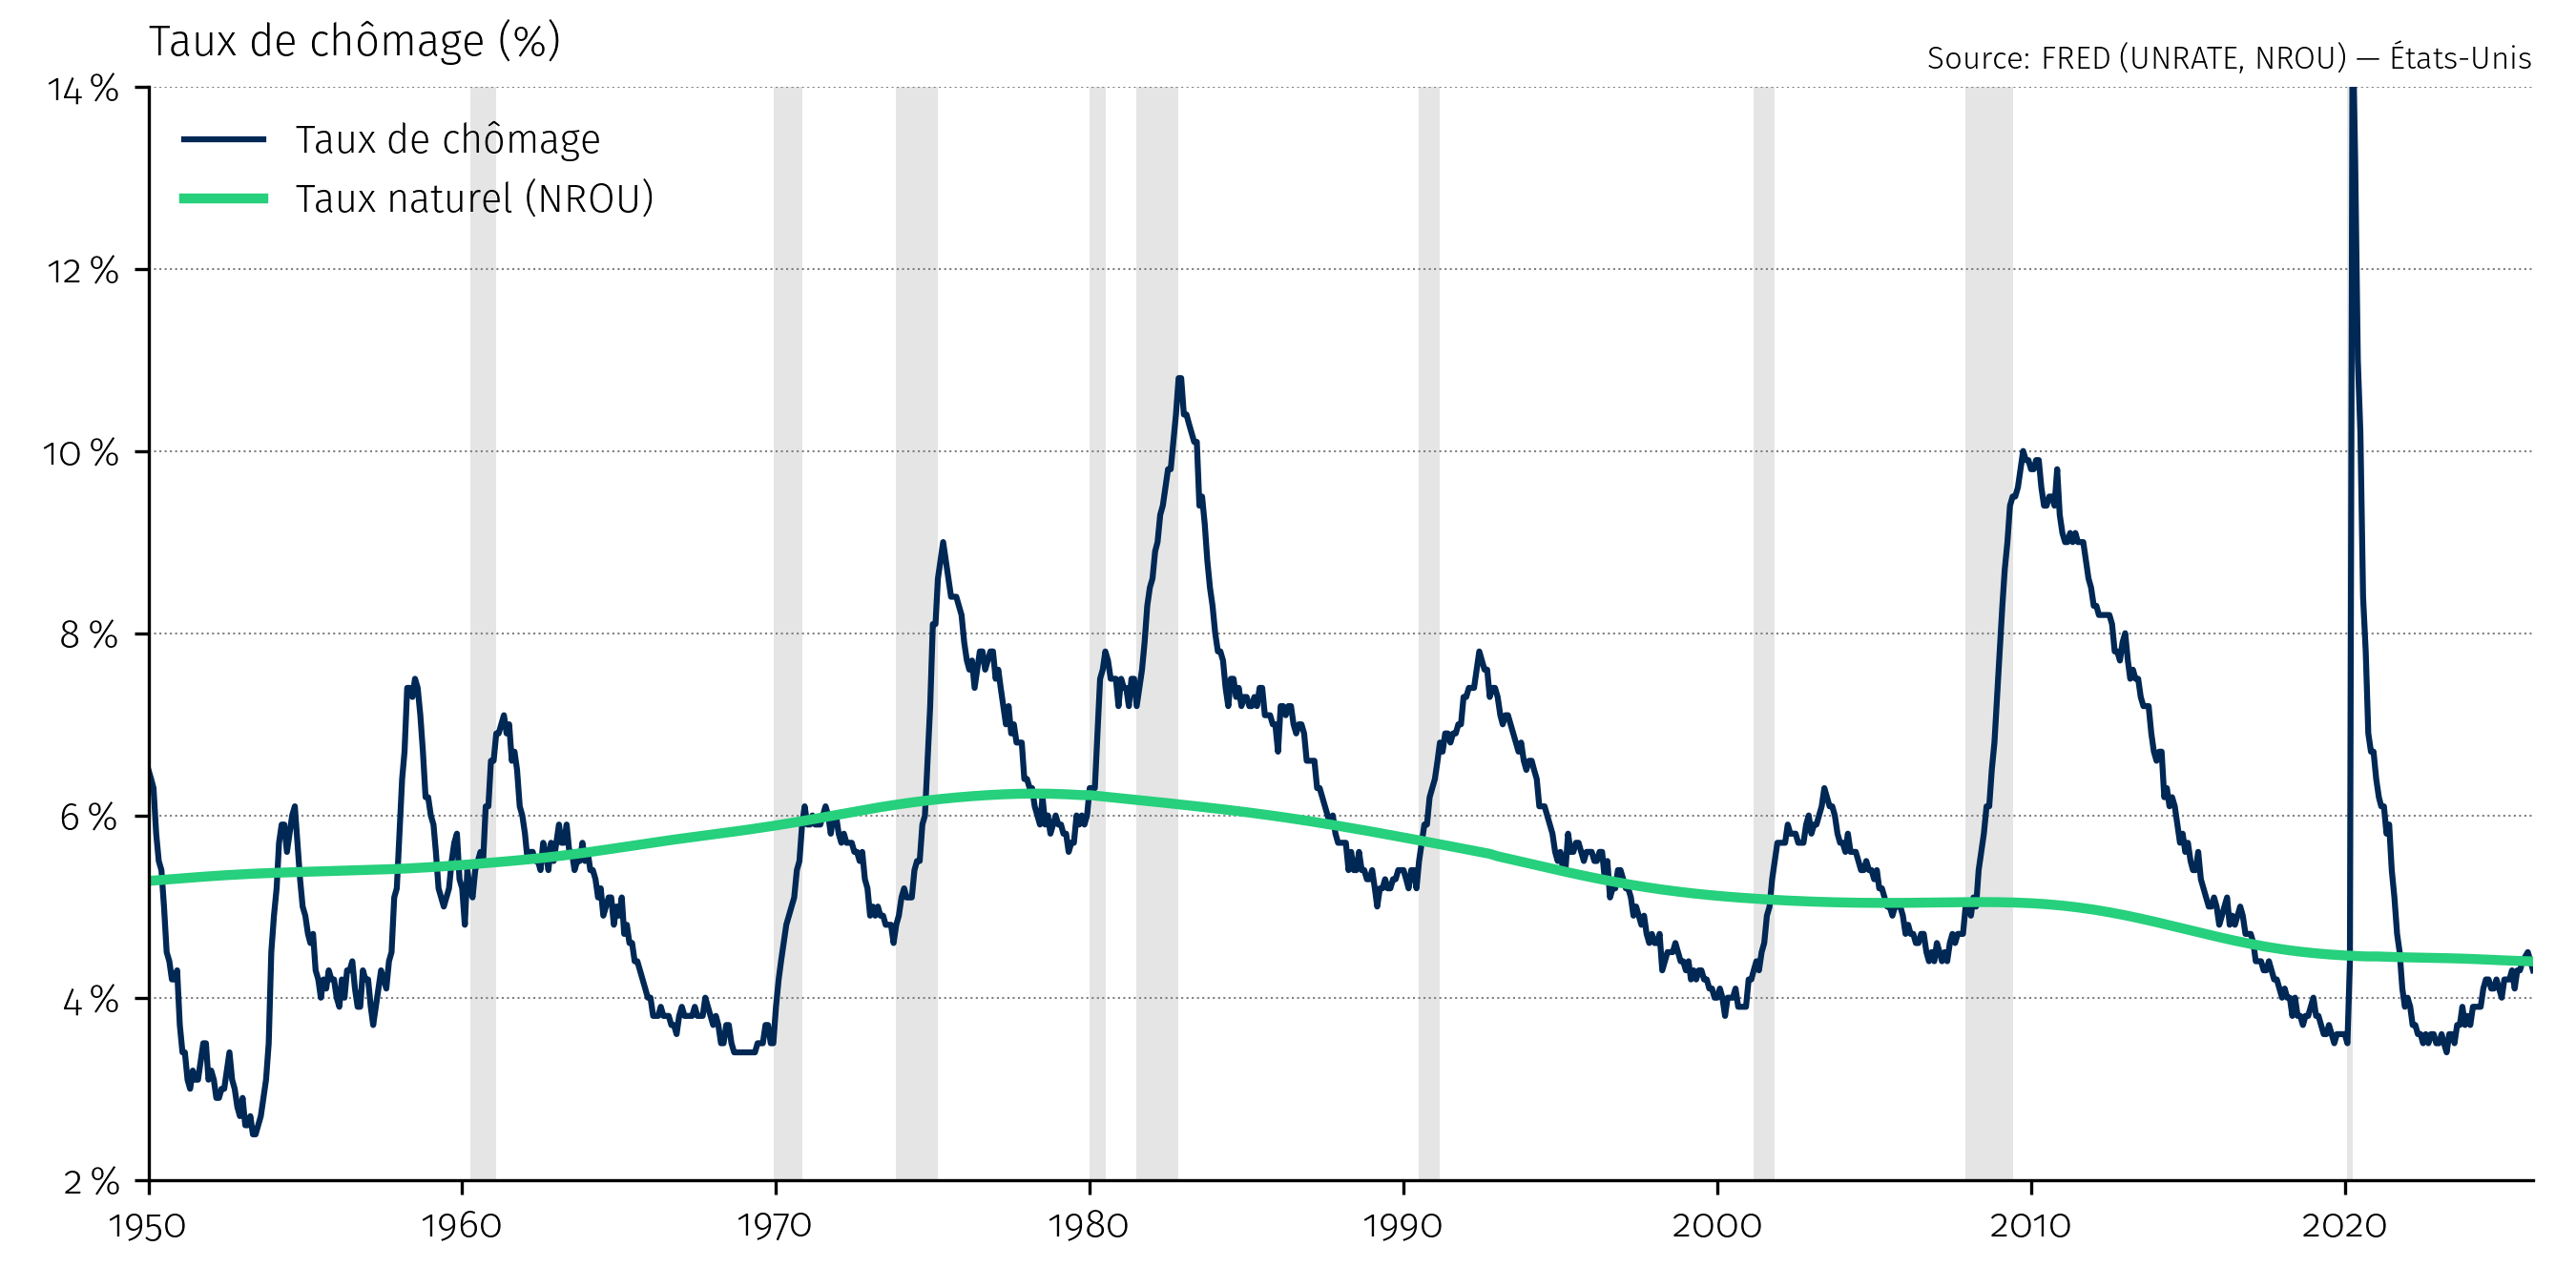
\includegraphics[width=0.95\textwidth, keepaspectratio]{natural_unemployment_usa.png}
   \end{figure}
\end{frame}

\begin{frame}[t]{PIB potentiel et écart de production}
   \small
   \begin{defbox}
      \vspace{-0.5cm}
      \begin{itemize}
         \setlength\itemsep{0.15cm}
         \item \textbf{PIB potentiel} ($Y^{\text{POT}}$) --- le niveau de production lorsque les facteurs sont utilisés à leur \textbf{capacité normale}. C'est la vitesse \guillemotleft~de croisière~\guillemotright.
         \item \textbf{Écart de production} --- mesure l'écart (en \%) entre le PIB réel et potentiel :
         \begin{equation*}
            \text{Écart de production} = \frac{Y - Y^{\text{POT}}}{Y^{\text{POT}}} \times 100
         \end{equation*}
      \end{itemize}
   \end{defbox}
   \vspace{0.1cm}
   \begin{itemize}
      \setlength\itemsep{0.15cm}
      \item \textbf{Récession :} écart négatif ($Y < Y^{\text{POT}}$)
      \item \textbf{Surchauffe :} écart positif ($Y > Y^{\text{POT}}$)
      \item \textbf{Plein emploi :} écart nul ($Y = Y^{\text{POT}}$)
   \end{itemize}
\end{frame}

\begin{frame}{Le PIB réel et potentiel du Canada}
   \begin{figure}
      \centering
      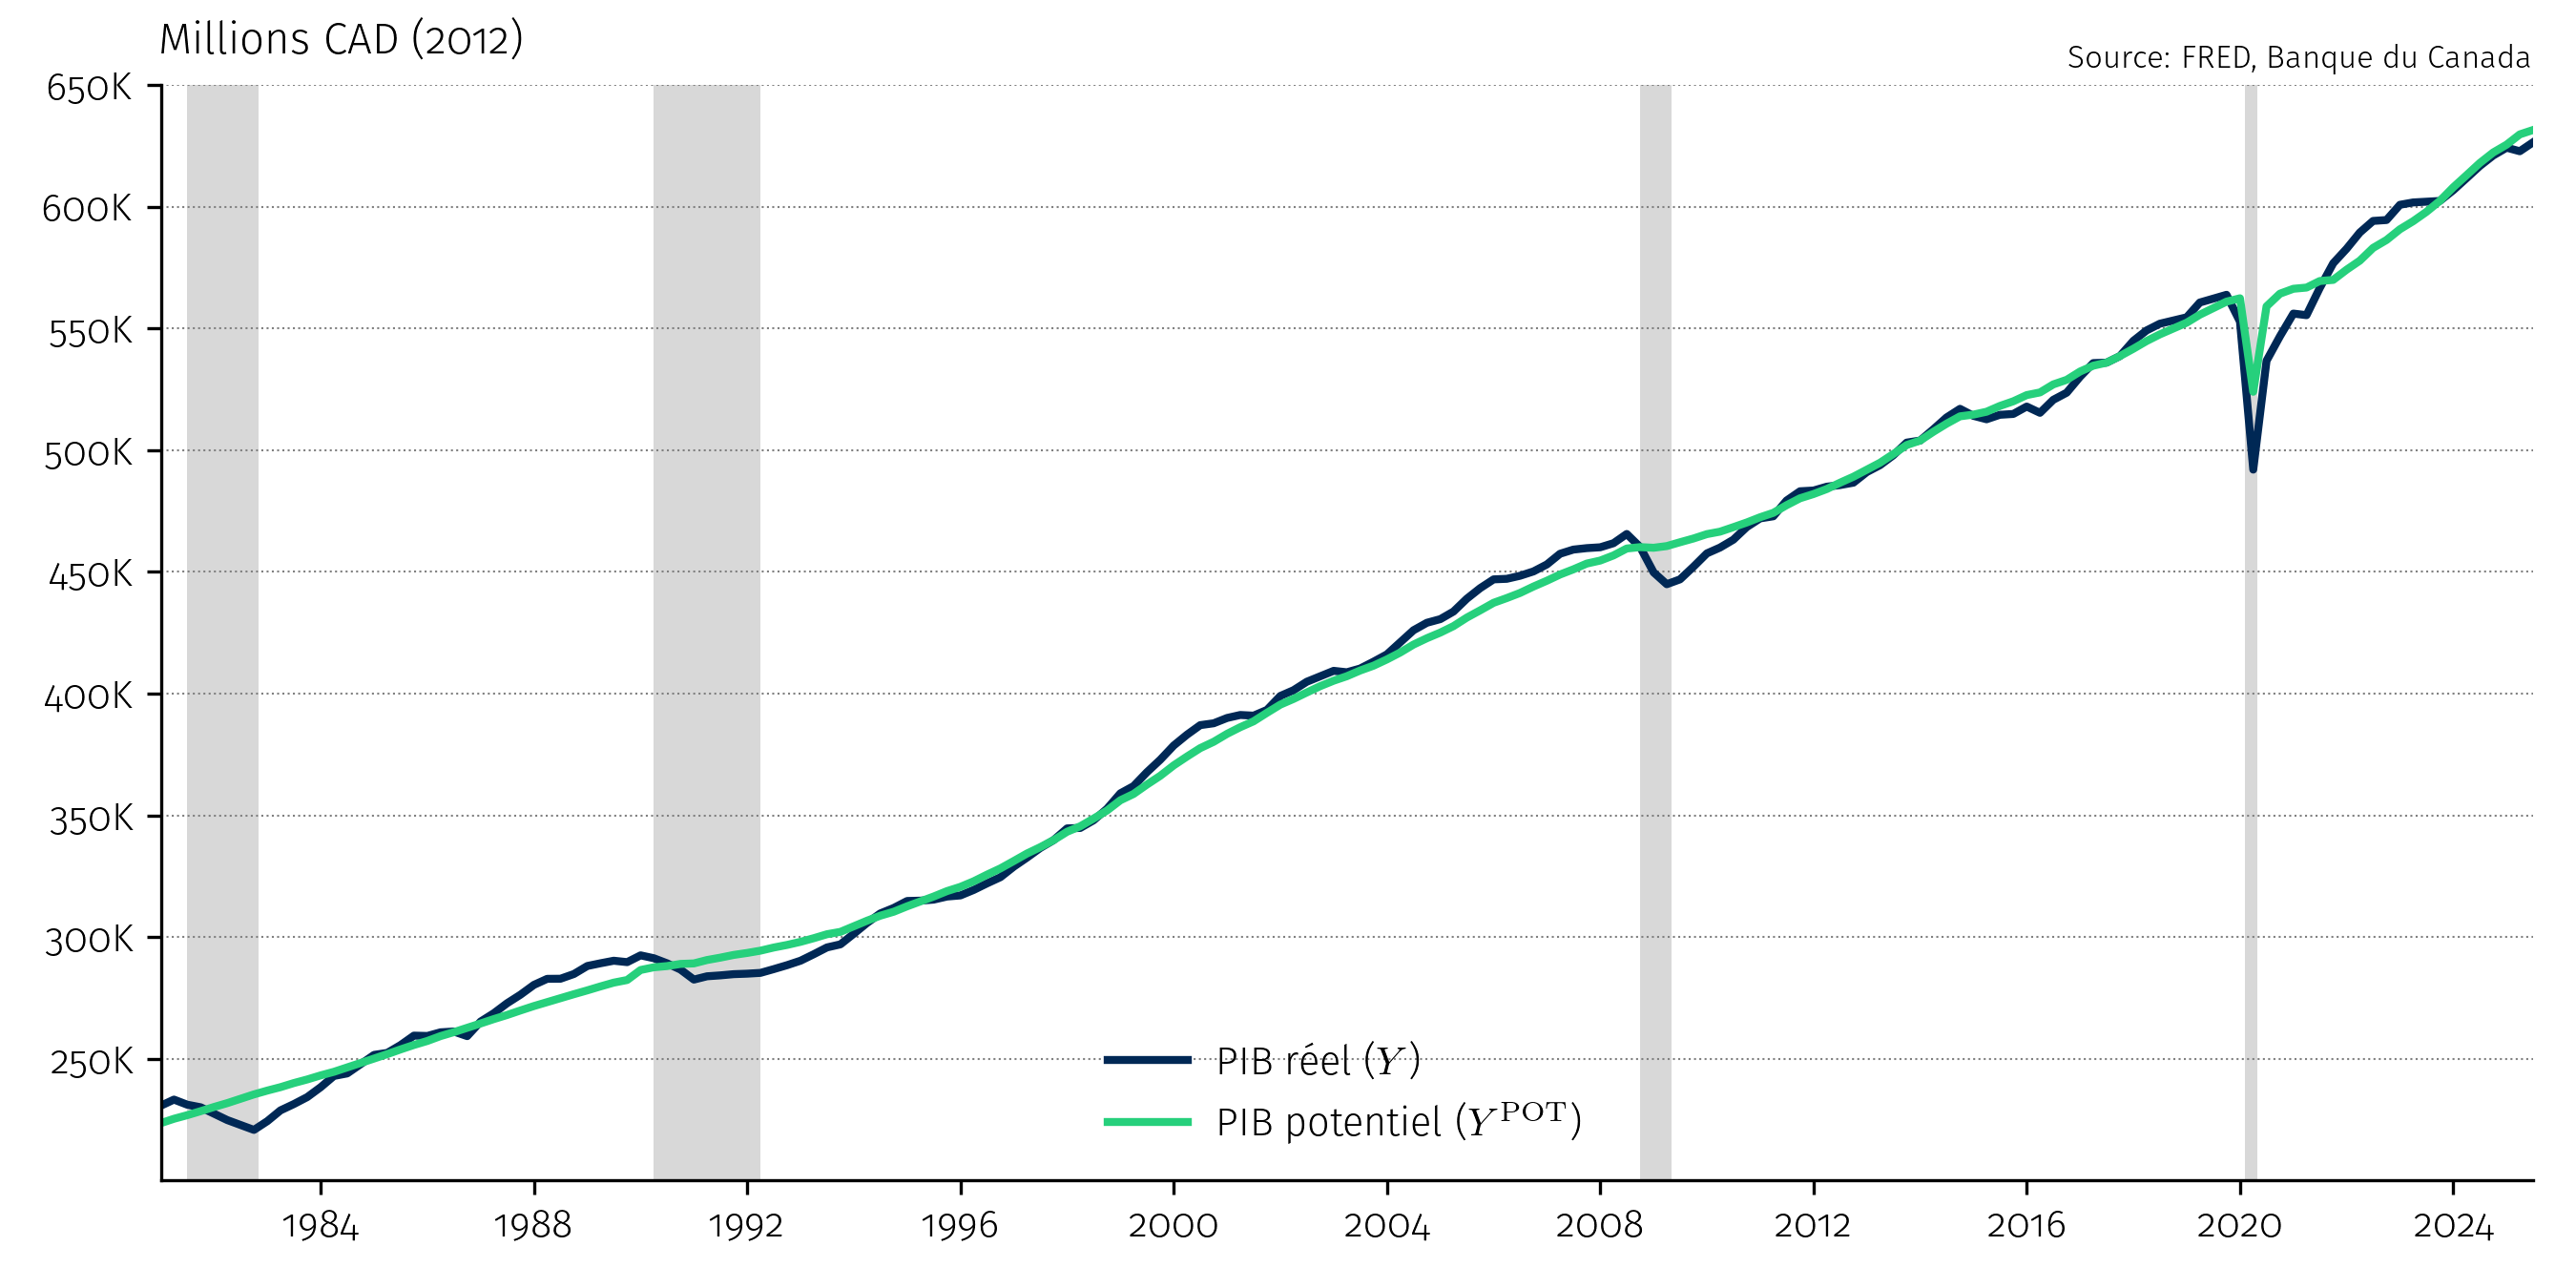
\includegraphics[width=0.95\textwidth, keepaspectratio]{canada_gdp_potential.png}
   \end{figure}
\end{frame}

\begin{frame}{L'écart de production au Canada}
   \begin{figure}
      \centering
      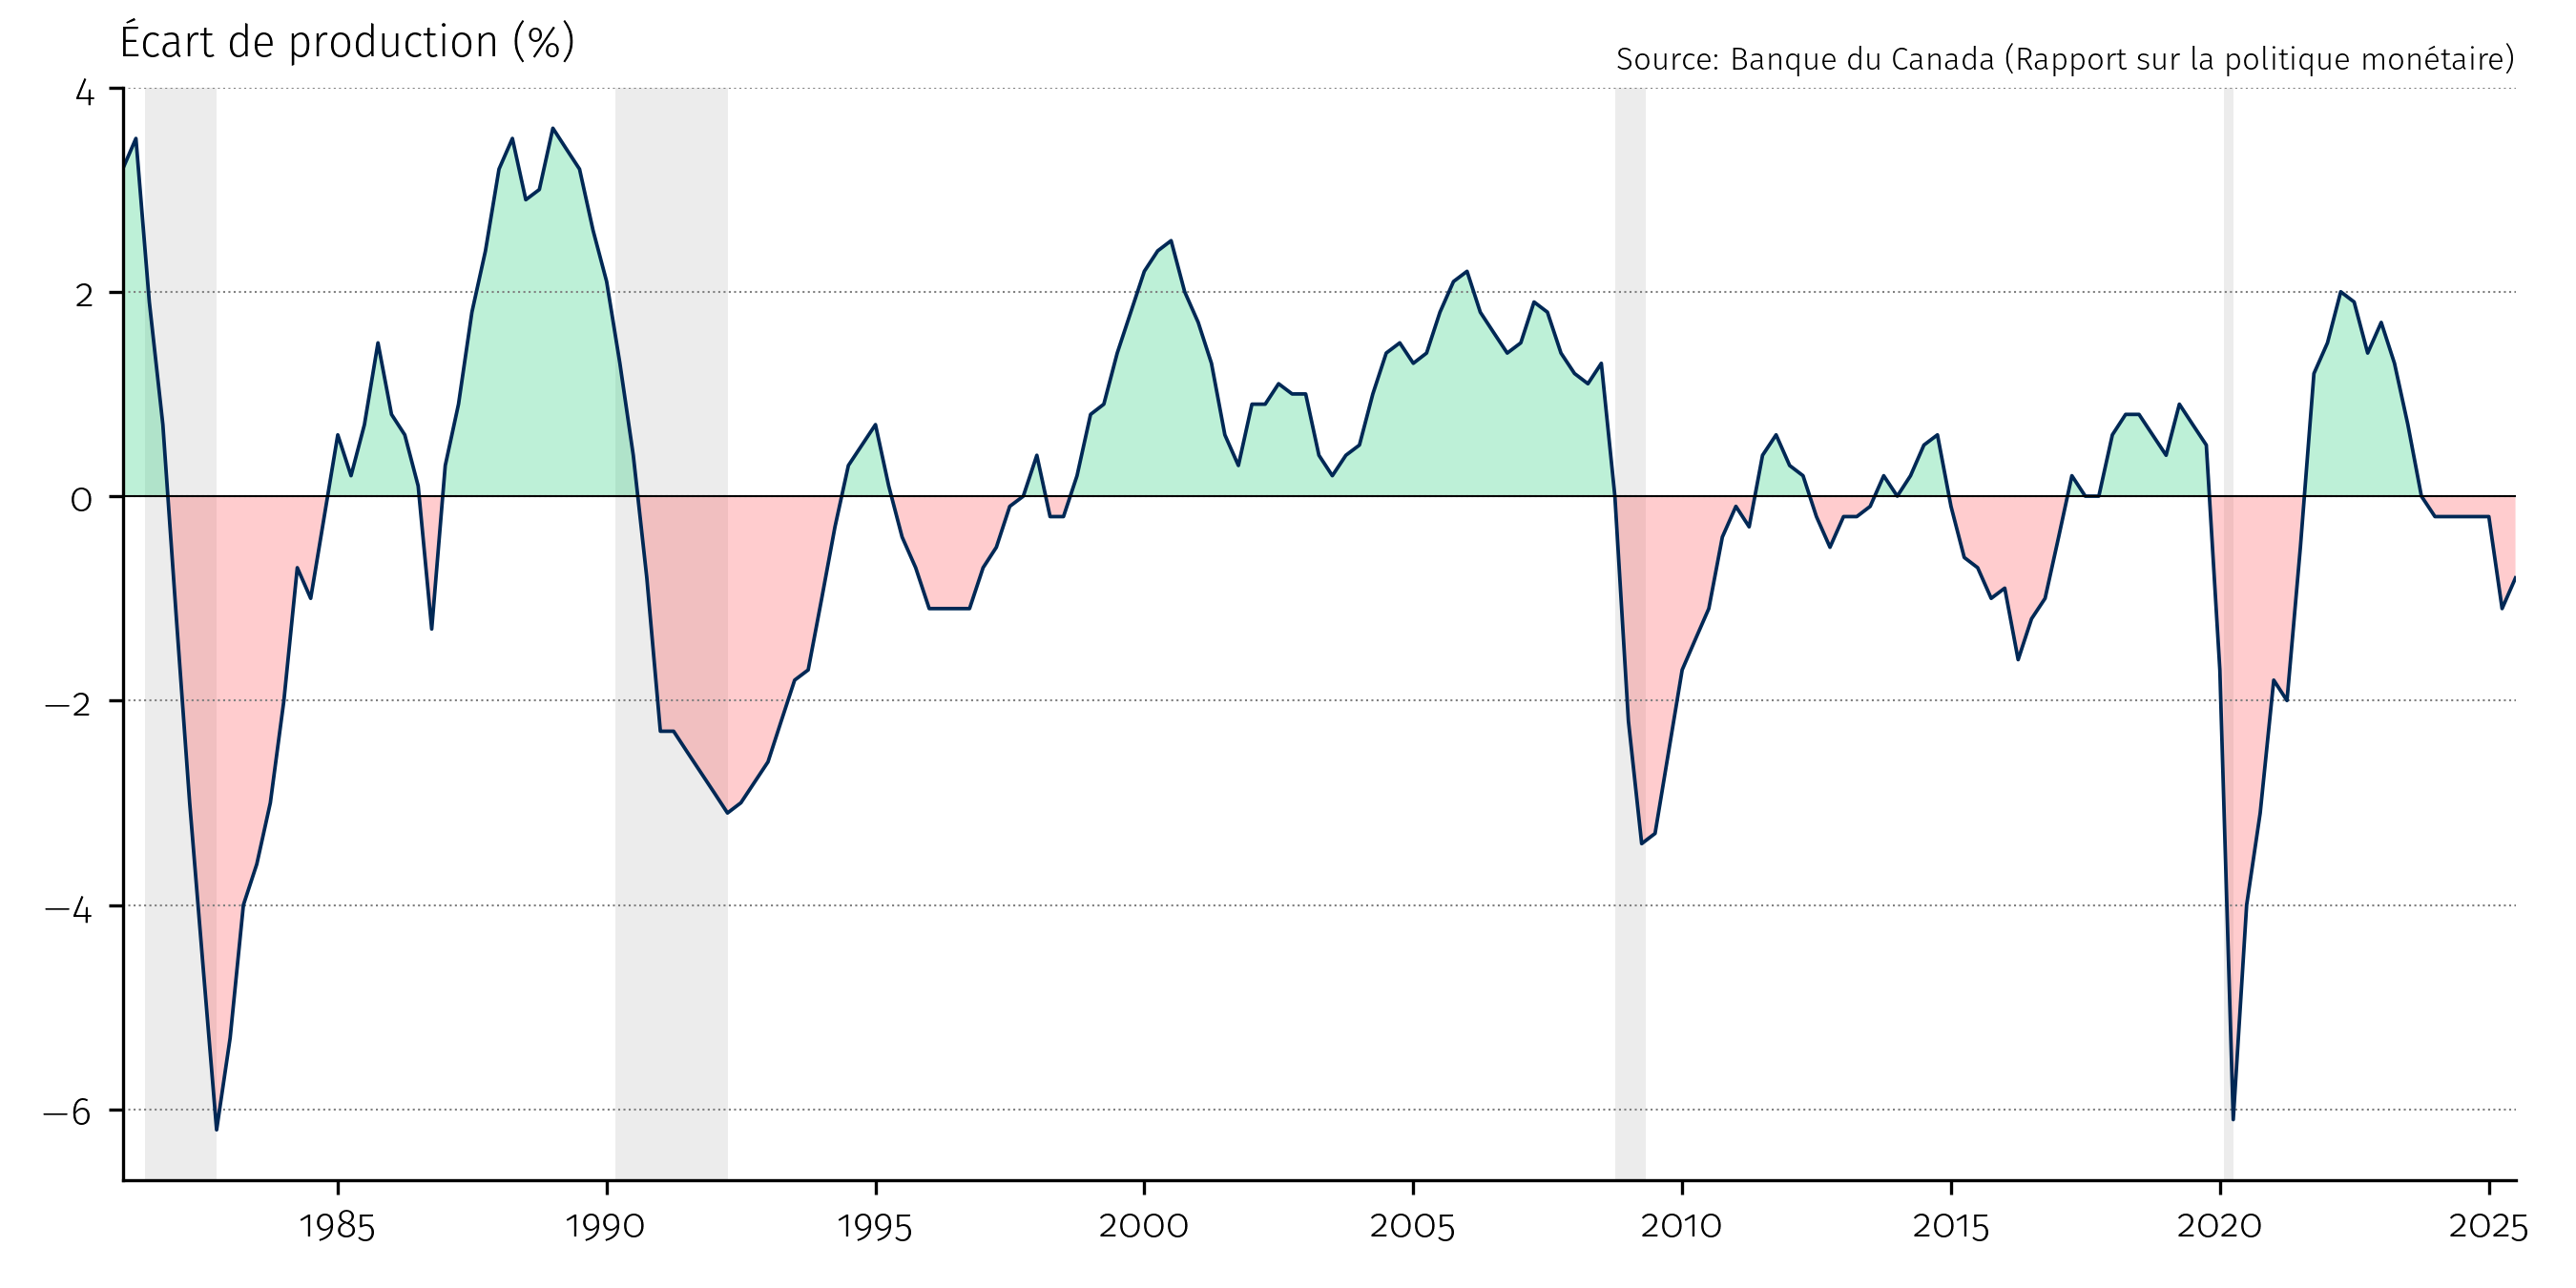
\includegraphics[width=0.95\textwidth, keepaspectratio]{output_gap_canada.png}
   \end{figure}
\end{frame}

% ============================================================================
\begin{frame}{Plan}
   \begin{enumerate}
      \setlength\itemsep{0.5cm}
      \item {\color{gray!50}Faits saillants sur les cycles économiques}
      \item {\color{gray!50}Tendance et fluctuations}
      \item \textbf{Le modèle AD-AS}
      \item Anatomie d'une récession
   \end{enumerate}
\end{frame}

% ============================================================================
\sectionframe{Le modèle AD-AS}
% ============================================================================

\begin{frame}[t]{Un cadre pour analyser les fluctuations}
   \small
   En microéconomie, on utilise l'offre et la demande pour analyser un marché particulier (sirop d'érable, pétrole, etc.). En macro, on fait la même chose --- mais pour l'\textbf{économie dans son ensemble}.

   \vspace{0.2cm}
   \begin{itemize}
      \setlength\itemsep{0.2cm}
      \item \textbf{Demande agrégée (AD)} --- quantités demandées par les ménages ($C$), les entreprises ($I$), le gouvernement ($G$) et le reste du monde ($NX$)
      \item \textbf{Offre agrégée (AS)} --- quantités produites par l'ensemble des entreprises
   \end{itemize}

   \vspace{0.2cm}
   \begin{bizimplication}[Ce cadre permet de répondre à des questions comme\ldots]
      \footnotesize
      \vspace{-0.5cm}
      \begin{itemize}
         \setlength\itemsep{0.05cm}
         \item Pourquoi la pandémie a-t-elle causé \textit{à la fois} une récession et de l'inflation?
         \item Pourquoi un choc pétrolier force la BdC à choisir entre inflation et chômage?
      \end{itemize}
   \end{bizimplication}
\end{frame}

\begin{frame}{Le diagramme AD-AS}
   \centering
   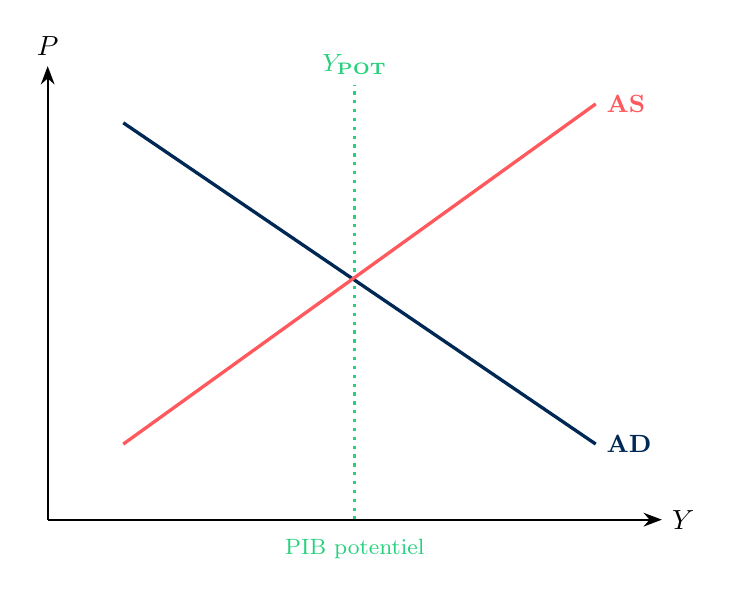
\begin{tikzpicture}[scale=1.2]
      % Potential GDP (vertical line)
      \draw[HECgreen, very thick, dotted] (3.25,0) -- (3.25,4.6)
         node[above, font=\small\bfseries, text=HECgreen] {$Y_{\text{POT}}$};
      \node[font=\footnotesize, text=HECgreen, below] at (3.25,-0.1) {PIB potentiel};
      % AD curve
      \draw[HECnavy, very thick] (0.8,4.2) -- (5.8,0.8)
         node[right, font=\small\bfseries, text=HECnavy] {AD};
      % AS curve
      \draw[HECcoral, very thick] (0.8,0.8) -- (5.8,4.4)
         node[right, font=\small\bfseries, text=HECcoral] {AS};
      % Axes
      \draw[-{Stealth}, thick] (0,0) -- (6.5,0) node[right] {$Y$};
      \draw[-{Stealth}, thick] (0,0) -- (0,4.8) node[above] {$P$};
   \end{tikzpicture}
\end{frame}

\begin{frame}[t]{La demande agrégée (AD)}
   \small
   \begin{columns}[T]
      \begin{column}{0.45\textwidth}
         \begin{defbox}[Demande agrégée]
            Relation entre niveau des prix ($P$) et niveau de dépenses ($Y$) :
            \vspace{0.15cm}

            \centering
            $Y = C + I + G + NX$
         \end{defbox}
         \vspace{0.3cm}
         \begin{keyinsight}
            Augmentation des prix $\to$ baisse de la quantité demandée.
         \end{keyinsight}
      \end{column}
      \begin{column}{0.52\textwidth}
         \centering
         \vspace{0.2cm}
         \begin{tikzpicture}[scale=1.15]
            % Axes
            \draw[-{Stealth}, thick] (0,0) -- (5.5,0) node[right] {$Y$};
            \draw[-{Stealth}, thick] (0,0) -- (0,4.5) node[above] {$P$};
            % AD curve
            \draw[HECnavy, very thick] (0.5,4) -- (5,0.5)
               node[right, font=\small\bfseries, text=HECnavy] {AD};
            % Points on the curve: y = 4 - (7/9)(x - 0.5)
            % At x=2: y=2.83, at x=4: y=1.28
            \filldraw[HECgreen!80!black] (4,1.28) circle (2.5pt);
            % Dotted reference lines
            \draw[dotted, HECgray] (2,0) node[below, font=\scriptsize] {$Y_1$} -- (2,2.83);
            \draw[dotted, HECgray] (0,2.83) node[left, font=\scriptsize] {$P_1$} -- (2,2.83);
            \draw[dotted, HECgray] (4,0) node[below, font=\scriptsize] {$Y_2$} -- (4,1.28);
            \draw[dotted, HECgray] (0,1.28) node[left, font=\scriptsize] {$P_2$} -- (4,1.28);
            % Arrow showing movement along curve
            \draw[-{Stealth[length=6pt]}, HECcoral, very thick] (2,2.83) -- (4,1.28);
            \filldraw[HECgreen!80!black] (2,2.83) circle (2.5pt);
         \end{tikzpicture}
      \end{column}
   \end{columns}
\end{frame}

\begin{frame}[t]{Ce qui déplace la courbe AD}
   \small
   Tout choc qui modifie les \textbf{dépenses souhaitées} à un niveau de prix donné :
   \vspace{0.5cm}
   \begin{columns}[T]
      \begin{column}{0.52\textwidth}
         \textbf{\textcolor{HECgreen}{Déplacements vers la droite}}
         \vspace{0.15cm}
         \begin{itemize}
            \setlength\itemsep{0.2cm}
            \item Hausse de la confiance ($C \uparrow$)
            \item Optimisme des entreprises ($I \uparrow$)
            \item Hausse des dépenses gouv.\ ($G \uparrow$)
            \item Boom d'exportations ($NX \uparrow$)
         \end{itemize}
         \vspace{0.2cm}
         {\footnotesize\textcolor{HECgray}{Les chocs inverses déplacent AD vers la gauche.}}
      \end{column}
      \begin{column}{0.46\textwidth}
         \centering
         \vspace{0.2cm}
         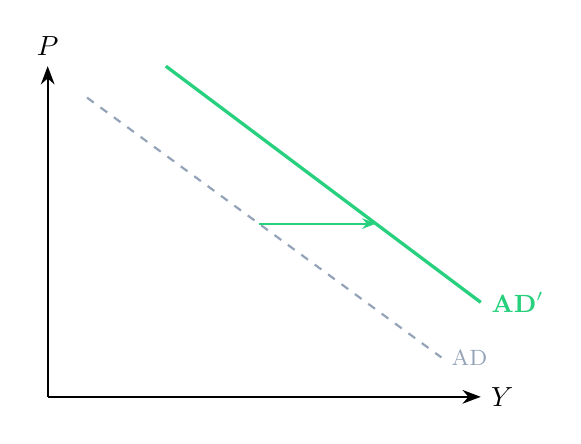
\begin{tikzpicture}[scale=1.0]
            % Axes
            \draw[-{Stealth}, thick] (0,0) -- (5.5,0) node[right] {$Y$};
            \draw[-{Stealth}, thick] (0,0) -- (0,4.2) node[above] {$P$};
            % Original AD (dashed gray)
            \draw[HECgray, dashed, thick] (0.5,3.8) -- (5,0.5)
               node[right, font=\footnotesize] {AD};
            % Shifted AD' (green, solid)
            \draw[HECgreen, very thick] (1.5,4.2) -- (5.5,1.2)
               node[right, font=\small\bfseries] {AD$'$};
            % Shift arrow: horizontal from AD to AD' at y=2.2
            \draw[-{Stealth[length=5pt]}, HECgreen, thick] (2.68,2.2) -- (4.17,2.2);
         \end{tikzpicture}
      \end{column}
   \end{columns}
\end{frame}

\begin{frame}[t]{L'offre agrégée (AS)}
   \small
   \begin{columns}[T]
      \begin{column}{0.45\textwidth}
         \begin{defbox}[Offre agrégée]
            Production des entreprises ($Y$) à un niveau des prix donné ($P$).
            \vspace{0.25cm}

            \textbf{Hypothèse clé :} les salaires nominaux sont rigides à court terme.
         \end{defbox}
         \vspace{0.25cm}
         \begin{keyinsight}
            À prix plus élevés $\to$ les firmes veulent produire davantage.
         \end{keyinsight}
      \end{column}
      \begin{column}{0.52\textwidth}
         \centering
         \vspace{0.2cm}
         \begin{tikzpicture}[scale=1.15]
            % Axes
            \draw[-{Stealth}, thick] (0,0) -- (5.5,0) node[right] {$Y$};
            \draw[-{Stealth}, thick] (0,0) -- (0,4.5) node[above] {$P$};
            % AS curve
            \draw[HECcoral, very thick] (0.5,0.5) -- (5,4)
               node[right, font=\small\bfseries, text=HECcoral] {AS};
            % Dotted reference lines
            \draw[dotted, HECgray] (1.5,0) node[below, font=\scriptsize] {$Y_1$} -- (1.5,1.28);
            \draw[dotted, HECgray] (0,1.28) node[left, font=\scriptsize] {$P_1$} -- (1.5,1.28);
            \draw[dotted, HECgray] (3.5,0) node[below, font=\scriptsize] {$Y_2$} -- (3.5,2.83);
            \draw[dotted, HECgray] (0,2.83) node[left, font=\scriptsize] {$P_2$} -- (3.5,2.83);
            % Arrow showing movement along curve
            % Points on the curve: y = 0.5 + (7/9)(x - 0.5)
            % At x=1.5: y=1.28, at x=3.5: y=2.83
            \filldraw[HECgreen!80!black] (3.5,2.83) circle (2.5pt);
            \draw[-{Stealth[length=6pt]}, HECnavy, very thick] (1.5,1.28) -- (3.5,2.83);
            \filldraw[HECgreen!80!black] (1.5,1.28) circle (2.5pt);
         \end{tikzpicture}
      \end{column}
   \end{columns}
\end{frame}

\begin{frame}[t]{Ce qui déplace la courbe AS}
   \small
   Tout ce qui modifie les \textbf{coûts de production} des entreprises à prix donnés :
   \vspace{0.5cm}
   \begin{columns}[T]
      \begin{column}{0.52\textwidth}
         \textbf{\textcolor{HECgreen}{Déplacements vers la droite}}
         \vspace{0.15cm}
         \begin{itemize}
            \setlength\itemsep{0.2cm}
            \item Progrès technologique ($A \uparrow$)
            \item Baisse du prix du pétrole
            \item Baisse des salaires nominaux
            \item Amélioration des chaînes d'approvisionnement
         \end{itemize}
         \vspace{0.2cm}
         {\footnotesize\textcolor{HECgray}{Les chocs inverses déplacent AS vers la gauche.}}
      \end{column}
      \begin{column}{0.46\textwidth}
         \centering
         \vspace{0.2cm}
         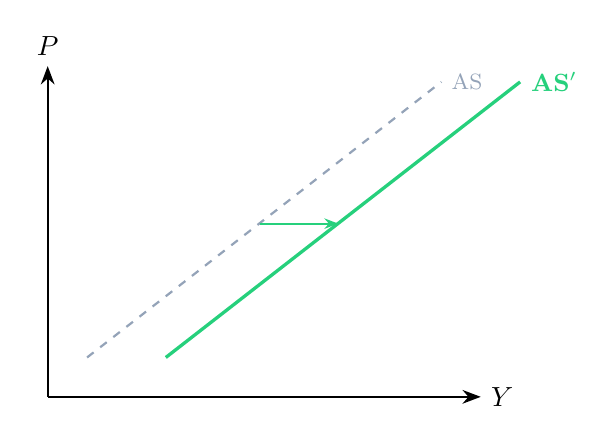
\begin{tikzpicture}[scale=1.0]
            % Axes
            \draw[-{Stealth}, thick] (0,0) -- (5.5,0) node[right] {$Y$};
            \draw[-{Stealth}, thick] (0,0) -- (0,4.2) node[above] {$P$};
            % Original AS (dashed gray)
            \draw[HECgray, dashed, thick] (0.5,0.5) -- (5,4)
               node[right, font=\footnotesize] {AS};
            % Shifted AS' (green, solid)
            \draw[HECgreen, very thick] (1.5,0.5) -- (6,4)
               node[right, font=\small\bfseries] {AS$'$};
            % Shift arrow: horizontal from AS to AS' at y=2.2
            % On AS: x = 0.5 + (9/7)(2.2 - 0.5) = 2.69
            % On AS': x = 1.5 + (9/7)(2.2 - 0.5) = 3.69
            \draw[-{Stealth[length=5pt]}, HECgreen, thick] (2.69,2.2) -- (3.69,2.2);
         \end{tikzpicture}
      \end{column}
   \end{columns}
\end{frame}

\begin{frame}{Équilibre de court terme}
   \centering
   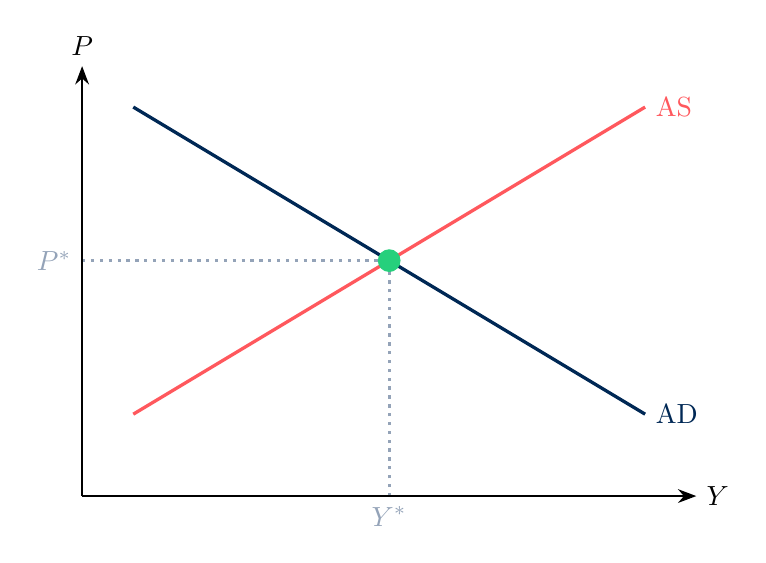
\begin{tikzpicture}[scale=1.3]
      % AD: y = -0.6x + 4.1
      \draw[HECnavy, very thick] (0.5,3.8) -- (5.5,0.8) node[right] {AD};
      % AS: y = 0.6x + 0.5
      \draw[HECcoral, very thick] (0.5,0.8) -- (5.5,3.8) node[right] {AS};
      % Intersection: -0.6x+4.1 = 0.6x+0.5 => x=3.0, y=2.3
      \draw[dotted, very thick, HECgray] (3.0,0) node[below] {$Y^*$} -- (3.0,2.3);
      \draw[dotted, very thick, HECgray] (0,2.3) node[left] {$P^*$} -- (3.0,2.3);
      \filldraw[HECgreen] (3.0,2.3) circle (3pt);
      % Axes
      \draw[-{Stealth}, thick] (0,0) -- (6,0) node[right] {$Y$};
      \draw[-{Stealth}, thick] (0,0) -- (0,4.2) node[above] {$P$};
   \end{tikzpicture}
\end{frame}

\begin{frame}[t]{Pourquoi ces pentes?}
   \footnotesize
   \vspace{0.2cm}
   \begin{columns}[T]
      \begin{column}{0.48\textwidth}
         \begin{tcolorbox}[
            colback=HECnavy!5, colframe=HECnavy, boxrule=0.5pt, arc=8pt,
            leftrule=3pt, top=6pt, bottom=6pt, left=8pt, right=8pt,
            title={\textcolor{HECnavy}{\textbf{AD : pente négative}}},
            coltitle=HECnavy, colbacktitle=HECnavy!12,
            equal height group=slopes
         ]
            \textbf{L'effet de richesse :}
            \begin{enumerate}
               \setlength\itemsep{0.12cm}
               \item Richesse des ménages en \$
               \item Hausse généralisée des prix
               \item Pouvoir d'achat $\downarrow$ $\to$ $C \downarrow$
            \end{enumerate}
            \vspace{0.2cm}
            \begin{tcolorbox}[
               colback=HECnavy!10, colframe=HECnavy!0, boxrule=0pt, arc=6pt,
               top=3pt, bottom=3pt, left=4pt, right=4pt
            ]
               \centering\bfseries
               $P \uparrow$ $\to$ richesse réelle $\downarrow$ $\to$ $C \downarrow$ $\to$ $Y \downarrow$
            \end{tcolorbox}
         \end{tcolorbox}
      \end{column}
      \begin{column}{0.48\textwidth}
         \begin{tcolorbox}[
            colback=HECcoral!5, colframe=HECcoral, boxrule=0.5pt, arc=8pt,
            leftrule=3pt, top=6pt, bottom=6pt, left=8pt, right=8pt,
            title={\textcolor{HECcoral}{\textbf{AS : pente positive}}},
            coltitle=HECcoral, colbacktitle=HECcoral!12,
            equal height group=slopes
         ]
            \textbf{L'effet des salaires rigides :}
            \begin{enumerate}
               \setlength\itemsep{0.12cm}
               \item Salaires nom. ($w$) fixés par contrat
               \item $P \uparrow$ mais $w$ fixe $\to$ coût réel $\downarrow$
               \item Production plus rentable $\to$ $Y \uparrow$
            \end{enumerate}
            \vspace{0.2cm}
            \begin{tcolorbox}[
               colback=HECcoral!10, colframe=HECcoral!0, boxrule=0pt, arc=6pt,
               top=3pt, bottom=3pt, left=4pt, right=4pt
            ]
               \centering\bfseries
               $P \uparrow$ $\to$ $w$ fixe $\to$ coût $\downarrow$ $\to$ $Y \uparrow$
            \end{tcolorbox}
         \end{tcolorbox}
      \end{column}
   \end{columns}
\end{frame}

% ============================================================================
\begin{frame}{Plan}
   \begin{enumerate}
      \setlength\itemsep{0.5cm}
      \item {\color{gray!50}Faits saillants sur les cycles économiques}
      \item {\color{gray!50}Tendance et fluctuations}
      \item {\color{gray!50}Le modèle AD-AS}
      \item \textbf{Anatomie d'une récession}
   \end{enumerate}
\end{frame}

% ============================================================================
\sectionframe{Anatomie d'une récession}
% ============================================================================

\begin{frame}{Anatomie d'une récession}
   Analyser une récession comme un \textbf{incendie} en quatre étapes :
   \vspace{0.3cm}
   \begin{enumerate}
      \setlength\itemsep{0.3cm}
      \item \textbf{Étincelle} --- ce qui déclenche la récession (\guillemotleft~le choc~\guillemotright)
      \item \textbf{Transmission} --- comment le choc se propage (AD, AS, ou les deux)
      \item \textbf{Carburant} --- ce qui amplifie la transmission
      \item \textbf{Pare-feu} --- la réponse politique visant à limiter les dégâts
   \end{enumerate}
   \vspace{0.3cm}
   \begin{bizimplication}[Application]
      Nous allons appliquer ce cadre à \textbf{deux récessions} : 2020 et 2026?
   \end{bizimplication}
\end{frame}

\begin{frame}[t]{1.\ L'étincelle}
   \small
   Trois grands types de chocs déclenchent les récessions :
   \vspace{0.25cm}
   \begin{enumerate}
      \setlength\itemsep{0.25cm}
      \item[\textcolor{HECnavy}{\textbf{A.}}] \textbf{Le faux pas} --- erreur de politique économique\\
         {\footnotesize\textcolor{HECgray}{Ex.\ : hausses de taux trop agressives, austérité prématurée}}
      \item[\textcolor{HECnavy}{\textbf{B.}}] \textbf{La gravité} --- ce qui monte doit redescendre\\
         {\footnotesize\textcolor{HECgray}{Ex.\ : bulles immobilières, bulles boursières}}
      \item[\textcolor{HECnavy}{\textbf{C.}}] \textbf{Le choc externe} --- événement imprévisible, exogène\\
         {\footnotesize\textcolor{HECgray}{Ex.\ : pandémie, embargo pétrolier, conflit géopolitique}}
   \end{enumerate}
   \vspace{0.3cm}
   \textbf{\textcolor{HECnavy}{Discussion :}}
   \vspace{0.1cm}
   \begin{itemize}
      \setlength\itemsep{0.1cm}
      \item Quelle étincelle pour la Grande Récession de 2008--09?
      \item Pour la récession de 2020?
   \end{itemize}
\end{frame}

% --- Application : La pandémie de 2020 ---
{
\setbeamertemplate{footline}{}
\begin{frame}{}
   \centering
   \vspace{2cm}
   {\LARGE\textbf{\textcolor{HECnavy}{Application : La pandémie de 2020}}}\\[12pt]
   {\large\textcolor{HECgray}{Étincelle : choc externe (type C)}}
\end{frame}
}

\begin{frame}{2.\ Transmission \textnormal{(1/3)} --- équilibre initial}
   \centering
   \vspace{0.1cm}
   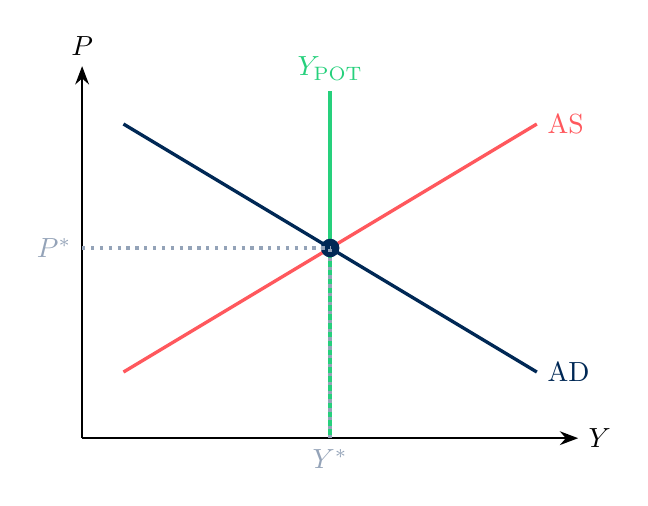
\begin{tikzpicture}[scale=1.05]
      % Axes
      \draw[-{Stealth}, thick] (0,0) -- (6,0) node[right] {$Y$};
      \draw[-{Stealth}, thick] (0,0) -- (0,4.5) node[above] {$P$};
      % Y_POT (vertical)
      \draw[HECgreen, very thick] (3.0,0) -- (3.0,4.2)
         node[above] {$Y_{\text{POT}}$};
      % AS: y = 0.6x + 0.5
      \draw[HECcoral, very thick] (0.5,0.8) -- (5.5,3.8) node[right] {AS};
      % AD: y = -0.6x + 4.1
      \draw[HECnavy, very thick] (0.5,3.8) -- (5.5,0.8) node[right] {AD};
      % Equilibrium at (3.0, 2.3)
      \filldraw[HECnavy] (3.0,2.3) circle (3pt);
      \draw[dotted, very thick, HECgray] (3.0,0) node[below] {$Y^*$} -- (3.0,2.3);
      \draw[dotted, very thick, HECgray] (0,2.3) node[left] {$P^*$} -- (3.0,2.3);
   \end{tikzpicture}
\end{frame}

\begin{frame}[t]{2.\ Transmission \textnormal{(2/3)} --- effondrement de la demande}
   \vspace{0.5cm}
   \begin{columns}[c]
      \begin{column}{0.55\textwidth}
         \centering
         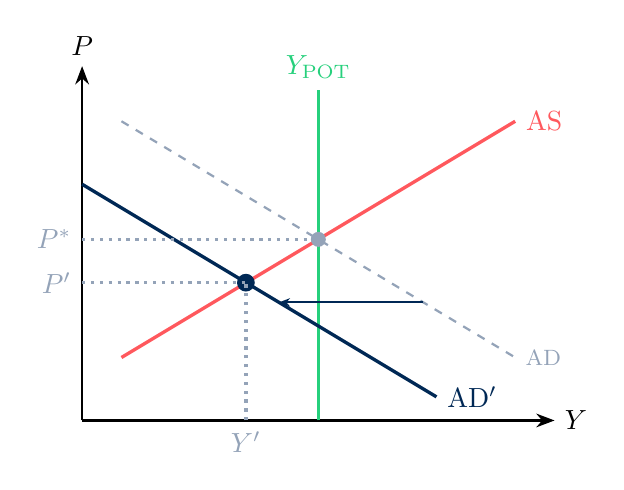
\begin{tikzpicture}[scale=1.0]
            % Axes
            \draw[-{Stealth}, thick] (0,0) -- (6,0) node[right] {$Y$};
            \draw[-{Stealth}, thick] (0,0) -- (0,4.5) node[above] {$P$};
            % Y_POT (vertical)
            \draw[HECgreen, very thick] (3.0,0) -- (3.0,4.2)
               node[above] {$Y_{\text{POT}}$};
            % AS: y = 0.6x + 0.5
            \draw[HECcoral, very thick] (0.5,0.8) -- (5.5,3.8) node[right] {AS};
            % AD original (dashed gray): y = -0.6x + 4.1
            \draw[HECgray, dashed, thick] (0.5,3.8) -- (5.5,0.8)
               node[right, font=\footnotesize] {AD};
            % AD' shifted left: y = -0.6x + 3.0
            \draw[HECnavy, very thick] (0.0,3.0) -- (4.5,0.3)
               node[right] {AD$'$};
            % Shift arrow (full span between AD and AD' at y=1.5)
            \draw[-{Stealth[length=4pt]}, HECnavy, thick] (4.33,1.5) -- (2.5,1.5);
            % Original equilibrium (faded) at (3.0, 2.3)
            \filldraw[HECgray] (3.0,2.3) circle (2.5pt);
            \draw[dotted, very thick, HECgray] (0,2.3) node[left] {$P^*$} -- (3.0,2.3);
            % New equilibrium: AD' ∩ AS at (2.08, 1.75)
            \filldraw[HECnavy] (2.08,1.75) circle (3pt);
            \draw[dotted, very thick, HECgray] (2.08,0) node[below] {$Y'$} -- (2.08,1.75);
            \draw[dotted, very thick, HECgray] (0,1.75) node[left] {$P'$} -- (2.08,1.75);
         \end{tikzpicture}
      \end{column}
      \begin{column}{0.42\textwidth}
         \small
         La \textbf{demande agrégée} s'effondre :
         \vspace{0.2cm}
         \begin{itemize}
            \setlength\itemsep{0.2cm}
            \item Effondrement de l'\textbf{investissement} ($I \downarrow$)
            \item Baisse de la \textbf{consommation} ($C \downarrow$) --- impossibilité de dépenser, précaution
         \end{itemize}
         \vspace{0.3cm}
         \textbf{AD se déplace vers la gauche}
         \vspace{0.2cm}

         {\footnotesize\textcolor{HECgray}{Résultat partiel : $Y \downarrow$ et $P \downarrow$}}
      \end{column}
   \end{columns}
\end{frame}

\begin{frame}[t]{2.\ Transmission \textnormal{(3/3)} --- un double choc rare}
   \vspace{0.5cm}
   \begin{columns}[c]
      \begin{column}{0.55\textwidth}
         \centering
         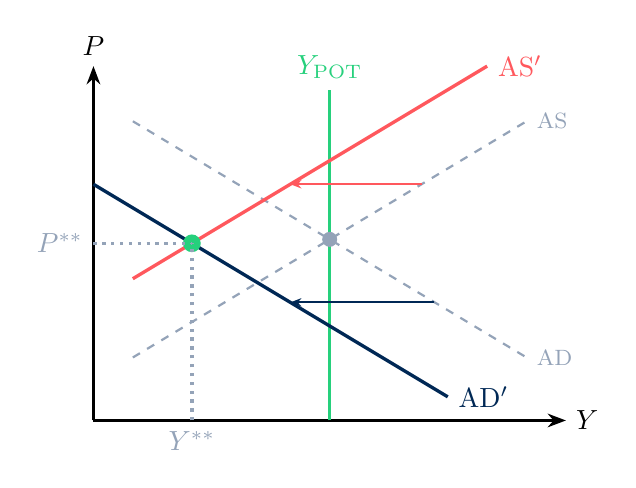
\begin{tikzpicture}[scale=1.0]
            % Axes
            \draw[-{Stealth}, thick] (0,0) -- (6,0) node[right] {$Y$};
            \draw[-{Stealth}, thick] (0,0) -- (0,4.5) node[above] {$P$};
            % Y_POT (vertical)
            \draw[HECgreen, very thick] (3.0,0) -- (3.0,4.2)
               node[above] {$Y_{\text{POT}}$};
            % AD original (dashed gray): y = -0.6x + 4.1
            \draw[HECgray, dashed, thick] (0.5,3.8) -- (5.5,0.8)
               node[right, font=\footnotesize] {AD};
            % AS original (dashed gray): y = 0.6x + 0.5
            \draw[HECgray, dashed, thick] (0.5,0.8) -- (5.5,3.8)
               node[right, font=\footnotesize] {AS};
            % AD' shifted left: y = -0.6x + 3.0
            \draw[HECnavy, very thick] (0.0,3.0) -- (4.5,0.3)
               node[right] {AD$'$};
            % AS' shifted left: y = 0.6x + 1.5
            \draw[HECcoral, very thick] (0.5,1.8) -- (5.0,4.5)
               node[right] {AS$'$};
            % Shift arrows
            \draw[-{Stealth[length=4pt]}, HECnavy, thick] (4.33,1.5) -- (2.5,1.5);
            \draw[-{Stealth[length=4pt]}, HECcoral, thick] (4.17,3.0) -- (2.5,3.0);
            % Original equilibrium (faded) at (3.0, 2.3)
            \filldraw[HECgray] (3.0,2.3) circle (2.5pt);
            % New equilibrium: AD' ∩ AS' at (1.25, 2.25)
            \filldraw[HECgreen] (1.25,2.25) circle (3pt);
            \draw[dotted, very thick, HECgray] (1.25,0) node[below] {$Y^{**}$} -- (1.25,2.25);
            \draw[dotted, very thick, HECgray] (0,2.25) node[left] {$P^{**}$} -- (1.25,2.25);
         \end{tikzpicture}
      \end{column}
      \begin{column}{0.42\textwidth}
         \small
         \textbf{L'offre agrégée} se contracte aussi :
         \vspace{0.15cm}
         \begin{itemize}
            \setlength\itemsep{0.15cm}
            \item \textbf{Confinements} $\to$ fermeture de la production (services)
            \item Perturbation des \textbf{chaînes d'approvisionnement}
         \end{itemize}
         \vspace{0.2cm}
         \textbf{AS se déplace aussi vers la gauche}
         \vspace{0.2cm}

         {\footnotesize\textcolor{HECgray}{Résultat : $Y \downarrow\downarrow$ (chocs se renforcent) et $P$ ambigu (effets opposés)}}
      \end{column}
   \end{columns}
\end{frame}

\begin{frame}[t]{3.\ Le carburant en 2020}
   \small
   \vspace{0.3cm}
   \begin{columns}[T]
      \begin{column}{0.48\textwidth}
         \textbf{Le carburant amplifie la transmission :}
         \vspace{0.15cm}
         \begin{itemize}
            \setlength\itemsep{0.15cm}
            \item \textbf{Accentue} le changement de comportement des acteurs
            \item Peut transformer un ralentissement en \textbf{récession majeure}
         \end{itemize}
      \end{column}
      \begin{column}{0.48\textwidth}
         \textbf{En 2020 :}
         \vspace{0.15cm}
         \begin{itemize}
            \setlength\itemsep{0.15cm}
            \item \textbf{Interdépendance mondiale} et complexification des chaînes d'approvisionnement
            \item \textit{Just-in-time} $\to$ fragilité
         \end{itemize}
      \end{column}
   \end{columns}
   \vspace{0.3cm}
   \begin{bizimplication}[Et au niveau micro?]
      Dans quelle mesure \textit{mon} organisation est-elle exposée aux chocs macro?
   \end{bizimplication}
\end{frame}

\begin{frame}{Le résultat : un effondrement record de l'emploi}
   \begin{figure}
      \centering
      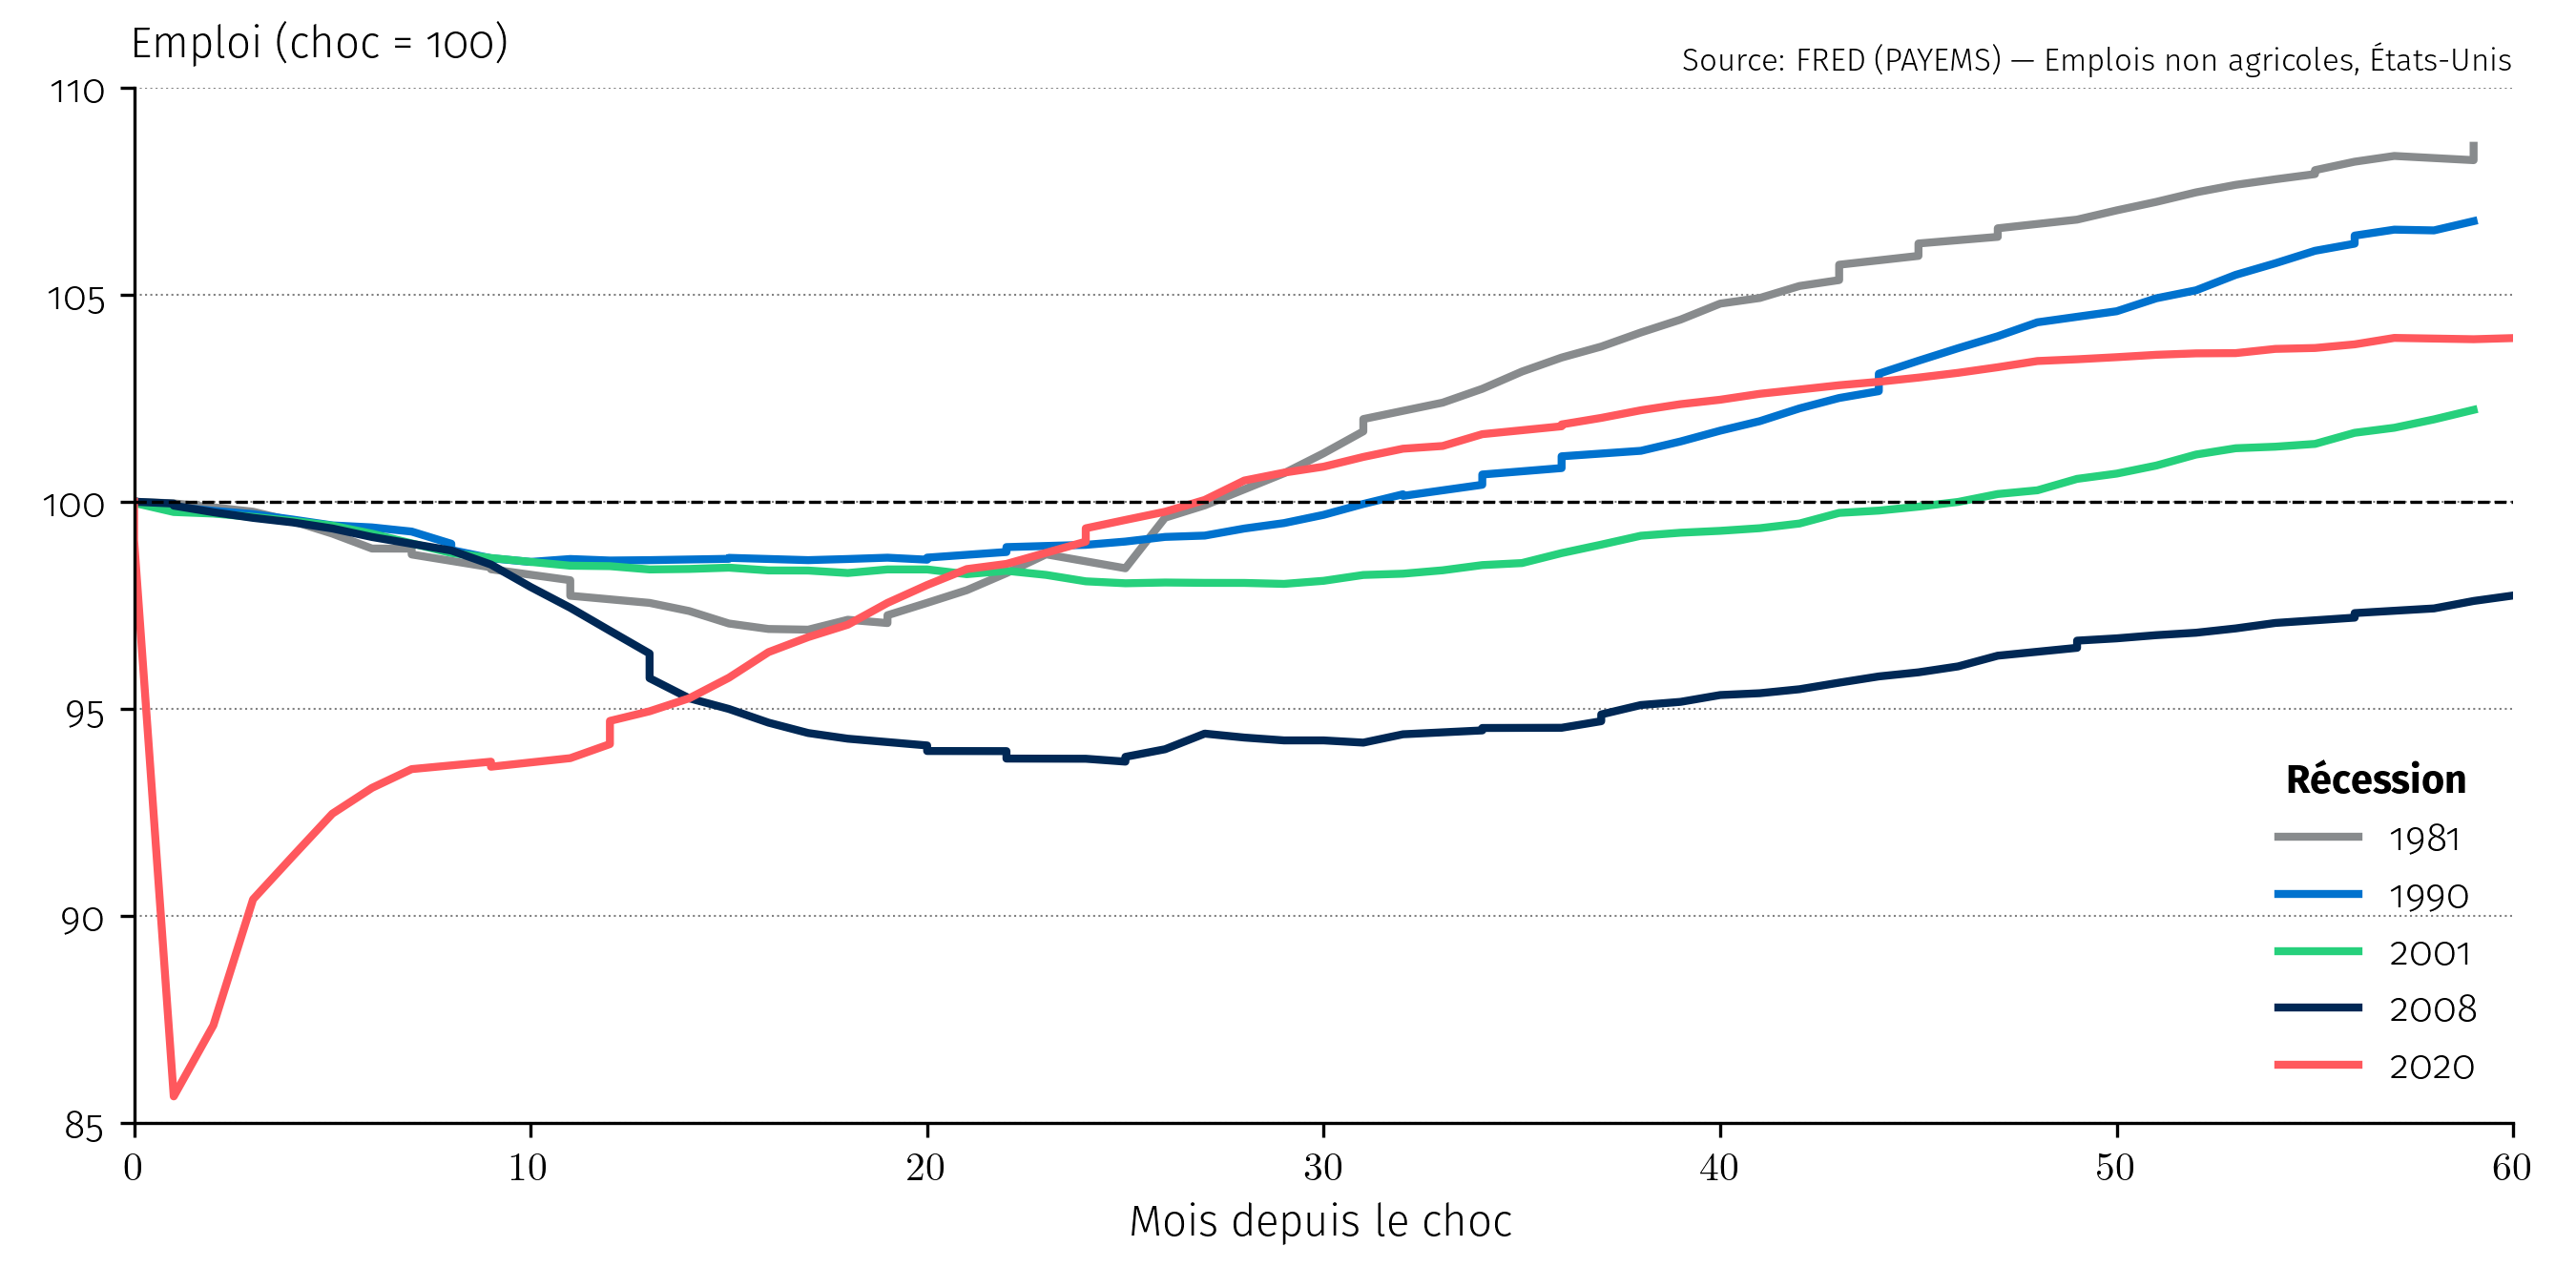
\includegraphics[width=0.95\textwidth, height=0.78\textheight, keepaspectratio]{employment_recovery.png}
   \end{figure}
\end{frame}

\begin{frame}{Le résultat : une baisse de l'inflation}
   \begin{figure}
      \centering
      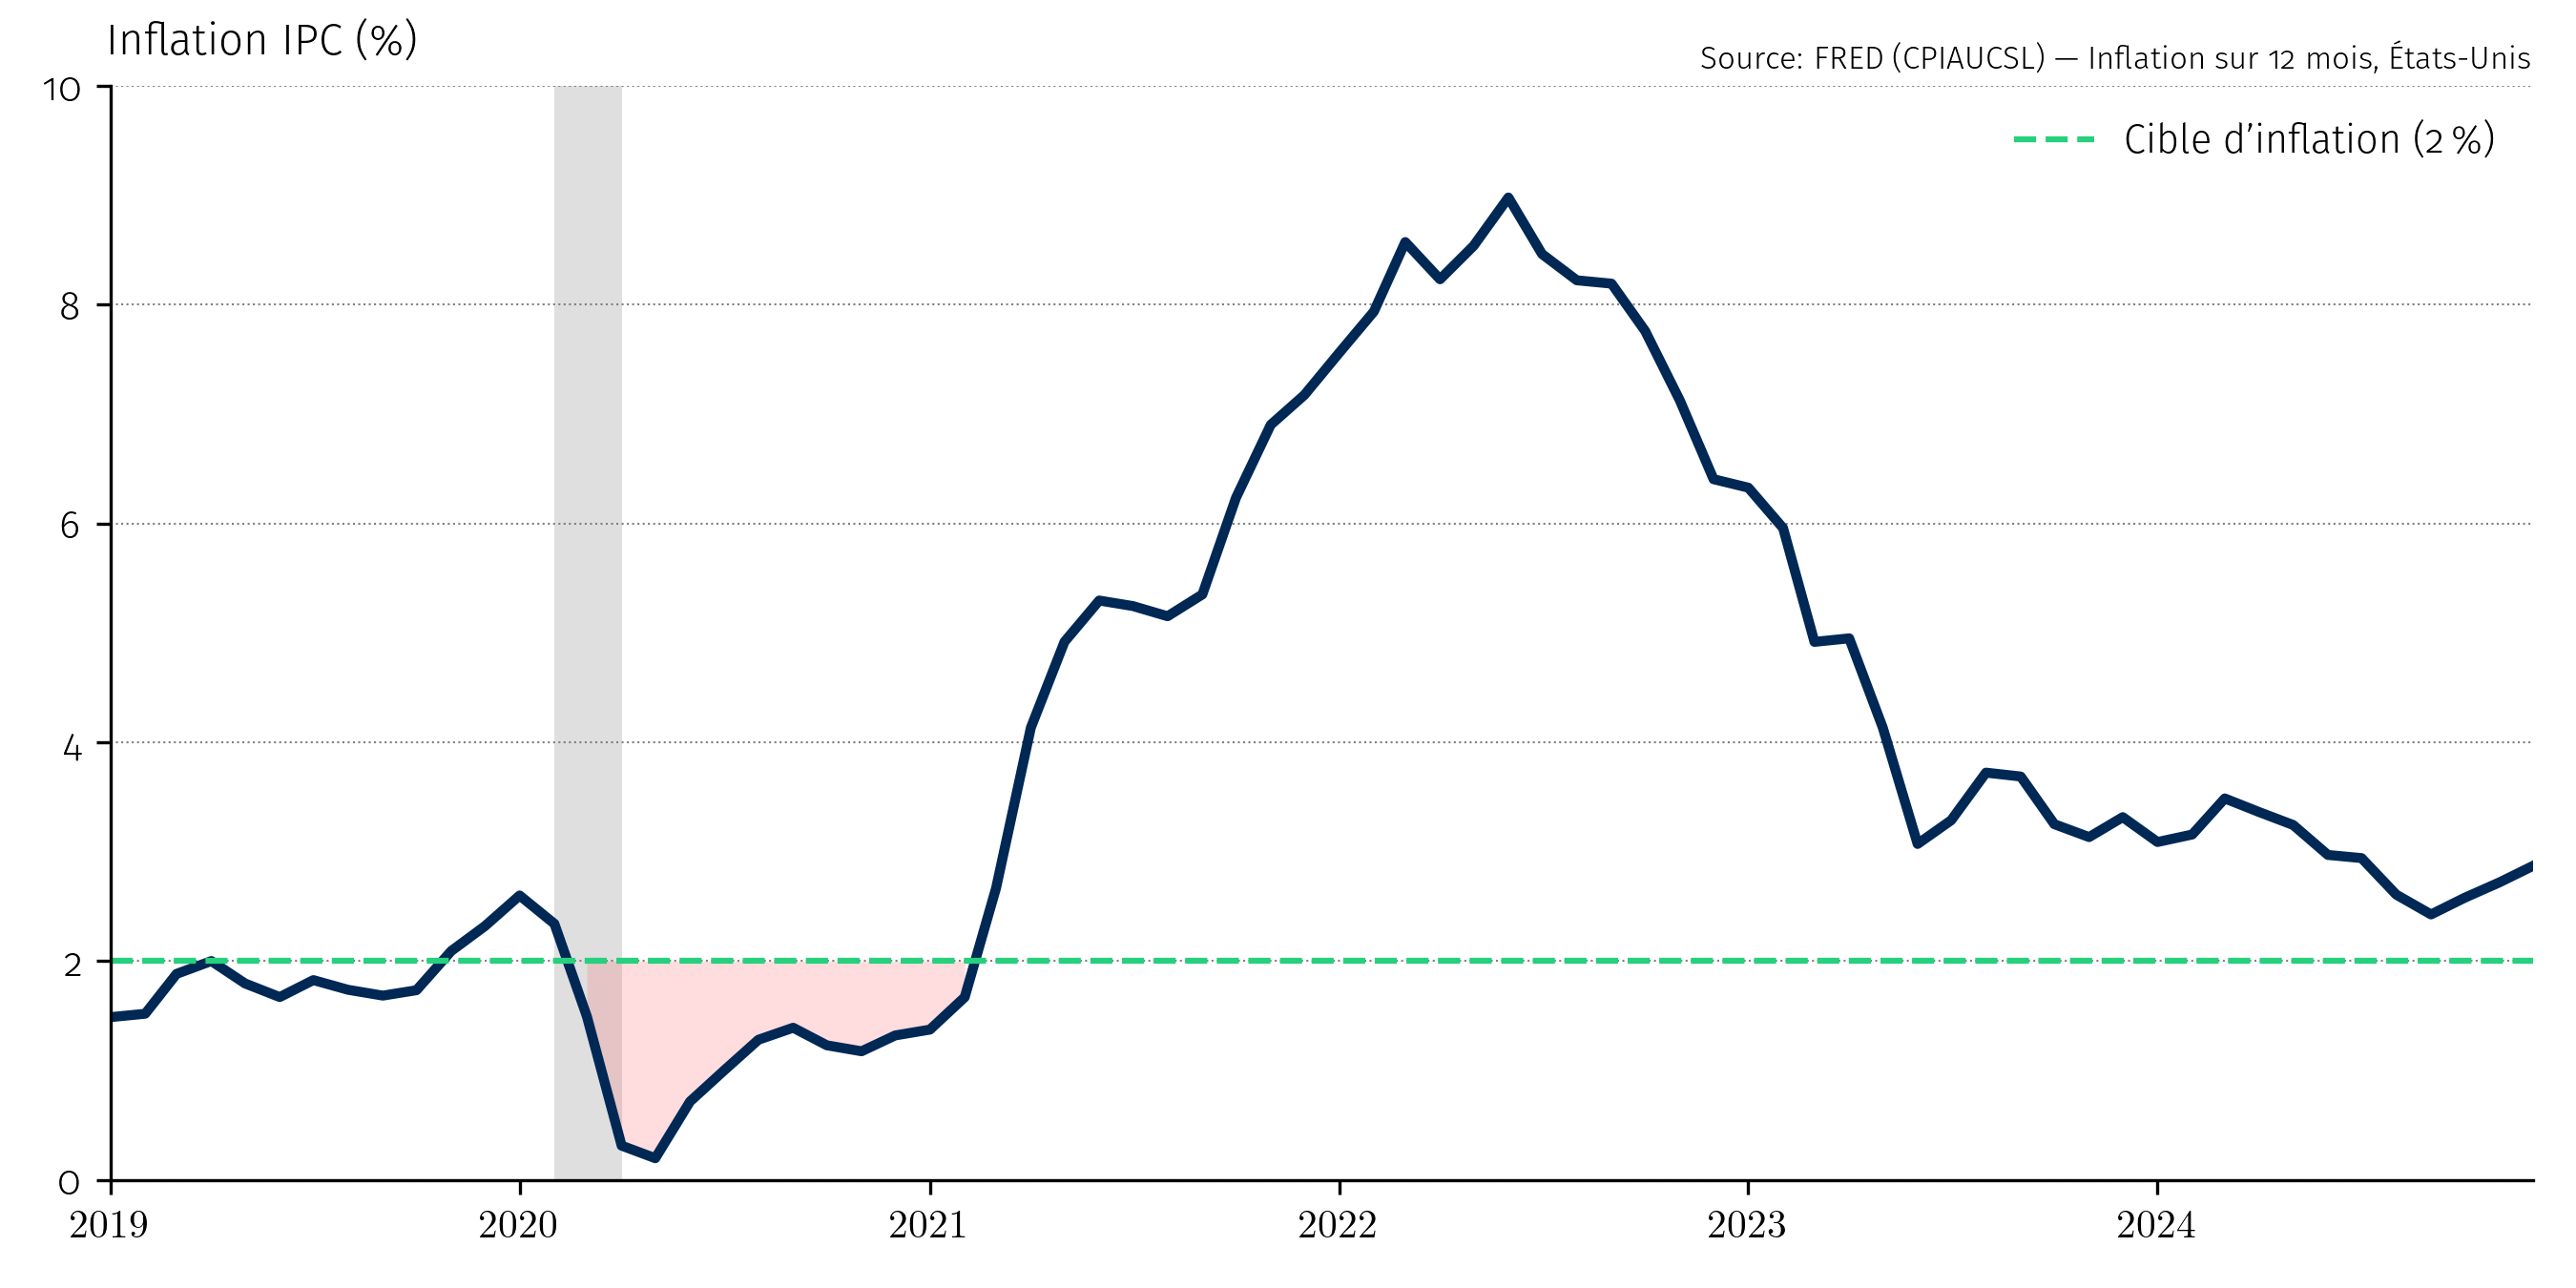
\includegraphics[width=0.95\textwidth, height=0.80\textheight, keepaspectratio]{us_recession_inflation.png}
   \end{figure}
\end{frame}

\begin{frame}{Pourquoi les prix baissent : AD domine AS}
   \centering
   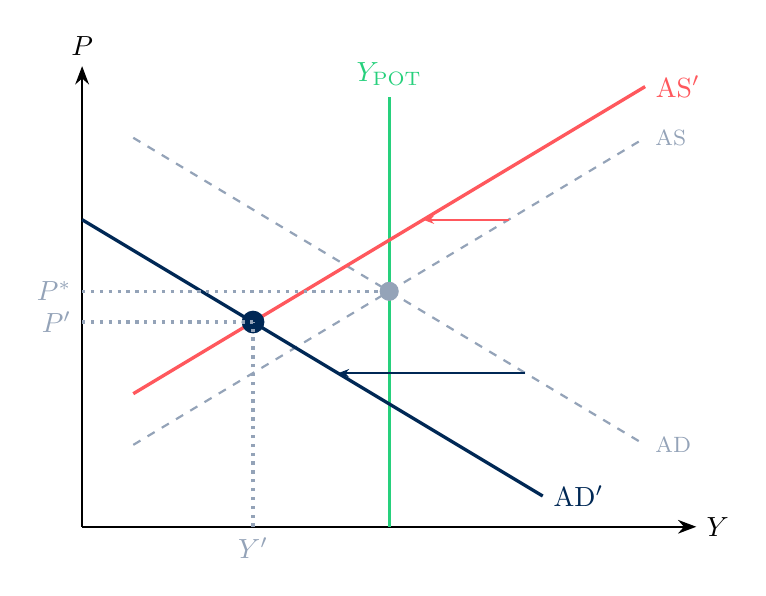
\begin{tikzpicture}[scale=1.3]
      % Axes
      \draw[-{Stealth}, thick] (0,0) -- (6,0) node[right] {$Y$};
      \draw[-{Stealth}, thick] (0,0) -- (0,4.5) node[above] {$P$};
      % Y_POT (vertical)
      \draw[HECgreen, very thick] (3.0,0) -- (3.0,4.2)
         node[above] {$Y_{\text{POT}}$};
      % AS original (dashed gray): y = 0.6x + 0.5
      \draw[HECgray, dashed, thick] (0.5,0.8) -- (5.5,3.8)
         node[right, font=\footnotesize] {AS};
      % AD original (dashed gray): y = -0.6x + 4.1
      \draw[HECgray, dashed, thick] (0.5,3.8) -- (5.5,0.8)
         node[right, font=\footnotesize] {AD};
      % AS' shifted left: y = 0.6x + 1.0
      \draw[HECcoral, very thick] (0.5,1.3) -- (5.5,4.3)
         node[right] {AS$'$};
      % AD' shifted further left: y = -0.6x + 3.0
      \draw[HECnavy, very thick] (0.0,3.0) -- (4.5,0.3)
         node[right] {AD$'$};
      % AD shift arrow (at y=1.5): from AD to AD'
      \draw[-{Stealth[length=4pt]}, HECnavy, thick] (4.33,1.5) -- (2.5,1.5);
      % AS shift arrow (at y=3.0): from AS to AS'
      \draw[-{Stealth[length=4pt]}, HECcoral, thick] (4.17,3.0) -- (3.33,3.0);
      % Original equilibrium (faded) at (3.0, 2.3)
      \filldraw[HECgray] (3.0,2.3) circle (2.5pt);
      \draw[dotted, very thick, HECgray] (0,2.3) node[left] {$P^*$} -- (3.0,2.3);
      % New equilibrium: AD' ∩ AS' at (1.67, 2.0)
      % -0.6x + 3.0 = 0.6x + 1.0 → 1.2x = 2.0 → x = 1.67, y = 2.0
      \filldraw[HECnavy] (1.67,2.0) circle (3pt);
      \draw[dotted, very thick, HECgray] (1.67,0) node[below] {$Y'$} -- (1.67,2.0);
      \draw[dotted, very thick, HECgray] (0,2.0) node[left] {$P'$} -- (1.67,2.0);
   \end{tikzpicture}
\end{frame}

\begin{frame}{Que s'est-il passé ensuite?}
   \centering
   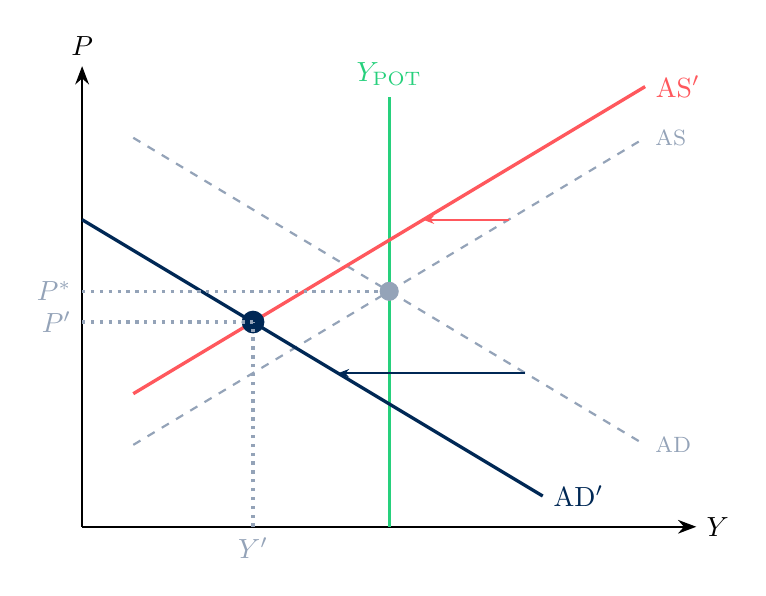
\begin{tikzpicture}[scale=1.3]
      % Axes
      \draw[-{Stealth}, thick] (0,0) -- (6,0) node[right] {$Y$};
      \draw[-{Stealth}, thick] (0,0) -- (0,4.5) node[above] {$P$};
      % Y_POT (vertical)
      \draw[HECgreen, very thick] (3.0,0) -- (3.0,4.2)
         node[above] {$Y_{\text{POT}}$};
      % AS original (dashed gray): y = 0.6x + 0.5
      \draw[HECgray, dashed, thick] (0.5,0.8) -- (5.5,3.8)
         node[right, font=\footnotesize] {AS};
      % AD original (dashed gray): y = -0.6x + 4.1
      \draw[HECgray, dashed, thick] (0.5,3.8) -- (5.5,0.8)
         node[right, font=\footnotesize] {AD};
      % AS' shifted left: y = 0.6x + 1.0
      \draw[HECcoral, very thick] (0.5,1.3) -- (5.5,4.3)
         node[right] {AS$'$};
      % AD' shifted further left: y = -0.6x + 3.0
      \draw[HECnavy, very thick] (0.0,3.0) -- (4.5,0.3)
         node[right] {AD$'$};
      % AD shift arrow (at y=1.5): from AD to AD'
      \draw[-{Stealth[length=4pt]}, HECnavy, thick] (4.33,1.5) -- (2.5,1.5);
      % AS shift arrow (at y=3.0): from AS to AS'
      \draw[-{Stealth[length=4pt]}, HECcoral, thick] (4.17,3.0) -- (3.33,3.0);
      % Original equilibrium (faded) at (3.0, 2.3)
      \filldraw[HECgray] (3.0,2.3) circle (2.5pt);
      \draw[dotted, very thick, HECgray] (0,2.3) node[left] {$P^*$} -- (3.0,2.3);
      % New equilibrium: AD' ∩ AS' at (1.67, 2.0)
      % -0.6x + 3.0 = 0.6x + 1.0 → 1.2x = 2.0 → x = 1.67, y = 2.0
      \filldraw[HECnavy] (1.67,2.0) circle (3pt);
      \draw[dotted, very thick, HECgray] (1.67,0) node[below] {$Y'$} -- (1.67,2.0);
      \draw[dotted, very thick, HECgray] (0,2.0) node[left] {$P'$} -- (1.67,2.0);
   \end{tikzpicture}
\end{frame}


% --- Application : Guerre en Iran (2026) ---
{
\setbeamertemplate{footline}{}
\begin{frame}{}
   \centering
   \vspace{2cm}
   {\LARGE\textbf{\textcolor{HECnavy}{Application :}}}\\[8pt]
   {\LARGE\textbf{\textcolor{HECnavy}{Guerre en Iran (2026)}}}\\[12pt]
   {\large\textcolor{HECgray}{Un choc d'offre en temps réel}}
\end{frame}
}

\begin{frame}[t]{Le coût macroéconomique des chocs pétroliers}
   \small
   \begin{defbox}[Règle approximative (FMI, Fed, BCE)]
      Hausse \textbf{persistante} de 10\,\% du prix du pétrole $\to$ PIB $-$\textbf{0.3 pp}, inflation $+$\textbf{0.4 pp}.
   \end{defbox}
   \vspace{0.1cm}
   \begin{itemize}
      \setlength\itemsep{0.15cm}
      \item[$\bullet$] \textbf{1973} (embargo OPEP, +300\,\%) : PIB É.-U.\ $-4.7$\,\%, Japon $-7$\,\%
      \item[$\bullet$] \textbf{1979} (révolution iranienne, +160\,\%) : PIB mondial $-3$\,\%
   \end{itemize}
   \vspace{0.1cm}
   \begin{bizimplication}[Asymétrie de Hamilton]
      Les hausses du pétrole font \textbf{plus de mal} que les baisses ne font de bien.
   \end{bizimplication}
\end{frame}

% --- Headline slide: Iran/Hormuz crisis ---
{
\setbeamertemplate{footline}{}
\begin{frame}{}
   \begin{tikzpicture}[remember picture, overlay]
      \setcounter{newshl}{0}
      \newsheadline[bloomberg]{Bloomberg}{\guillemotleft~Trump's Iran War Pushes World to the Brink of an Energy Crisis~\guillemotright}
      \newsheadline[washpost]{Washington Post}{\guillemotleft~Iran strikes stall traffic in Strait of Hormuz, rattling world markets~\guillemotright}
      \newsheadline[globeandmail]{The Globe and Mail}{\guillemotleft~Tanker attack in the northern Persian Gulf boosts oil and gas prices~\guillemotright}
      \newsheadline[radiocanada]{Radio-Canada}{\guillemotleft~Vers ``le scénario le plus toxique'' pour l'industrie pétrolière?~\guillemotright}
      \newsheadline[ft]{Financial Times}{\guillemotleft~Iran war triggers aluminium supply crunch and shutdowns across Middle East~\guillemotright}
      \newsheadline[economist]{The Economist}{\guillemotleft~The nightmare Iran energy scenario is becoming reality~\guillemotright}
   \end{tikzpicture}
\end{frame}
}

\begin{frame}[t]{28 février 2026 : Opération \textit{Epic Fury}}
   \footnotesize
   \textbf{L'étincelle :}
   \begin{itemize}
      \setlength\itemsep{0.05cm}
      \item[$\bullet$] Frappes coordonnées É.-U./Israël sur les sites nucléaires iraniens
      \item[$\bullet$] L'Iran riposte : 500+ missiles balistiques, 2\,000+ drones sur la région
      \item[$\bullet$] Frappes sur Dubaï, Abu Dhabi, Doha; QatarEnergy suspend sa production de GNL
   \end{itemize}
   \vspace{0.1cm}
   \textbf{Le blocage d'Ormuz :}
   \begin{itemize}
      \setlength\itemsep{0.05cm}
      \item[$\bullet$] $\sim$20\,\% du pétrole mondial transite par le détroit (20~M barils/jour)
      \item[$\bullet$] Les assureurs retirent la couverture de risque de guerre $\to$ transit impossible
      \item[$\bullet$] Maersk, Hapag-Lloyd suspendent tout passage; le trafic tombe à $\sim$zéro
   \end{itemize}
   \vspace{0.1cm}
   \begin{warning}[Choc d'offre $\neq$ choc de demande]
      En 2020, la demande s'est effondrée $\to$ désinflation. Ici, c'est l'\textbf{offre} qui se contracte $\to$ \textbf{stagflation} (prix $\uparrow$, production $\downarrow$).
   \end{warning}
\end{frame}

\begin{frame}{Le prix du Brent autour de l'opération Epic Fury}
   \begin{figure}
      \centering
      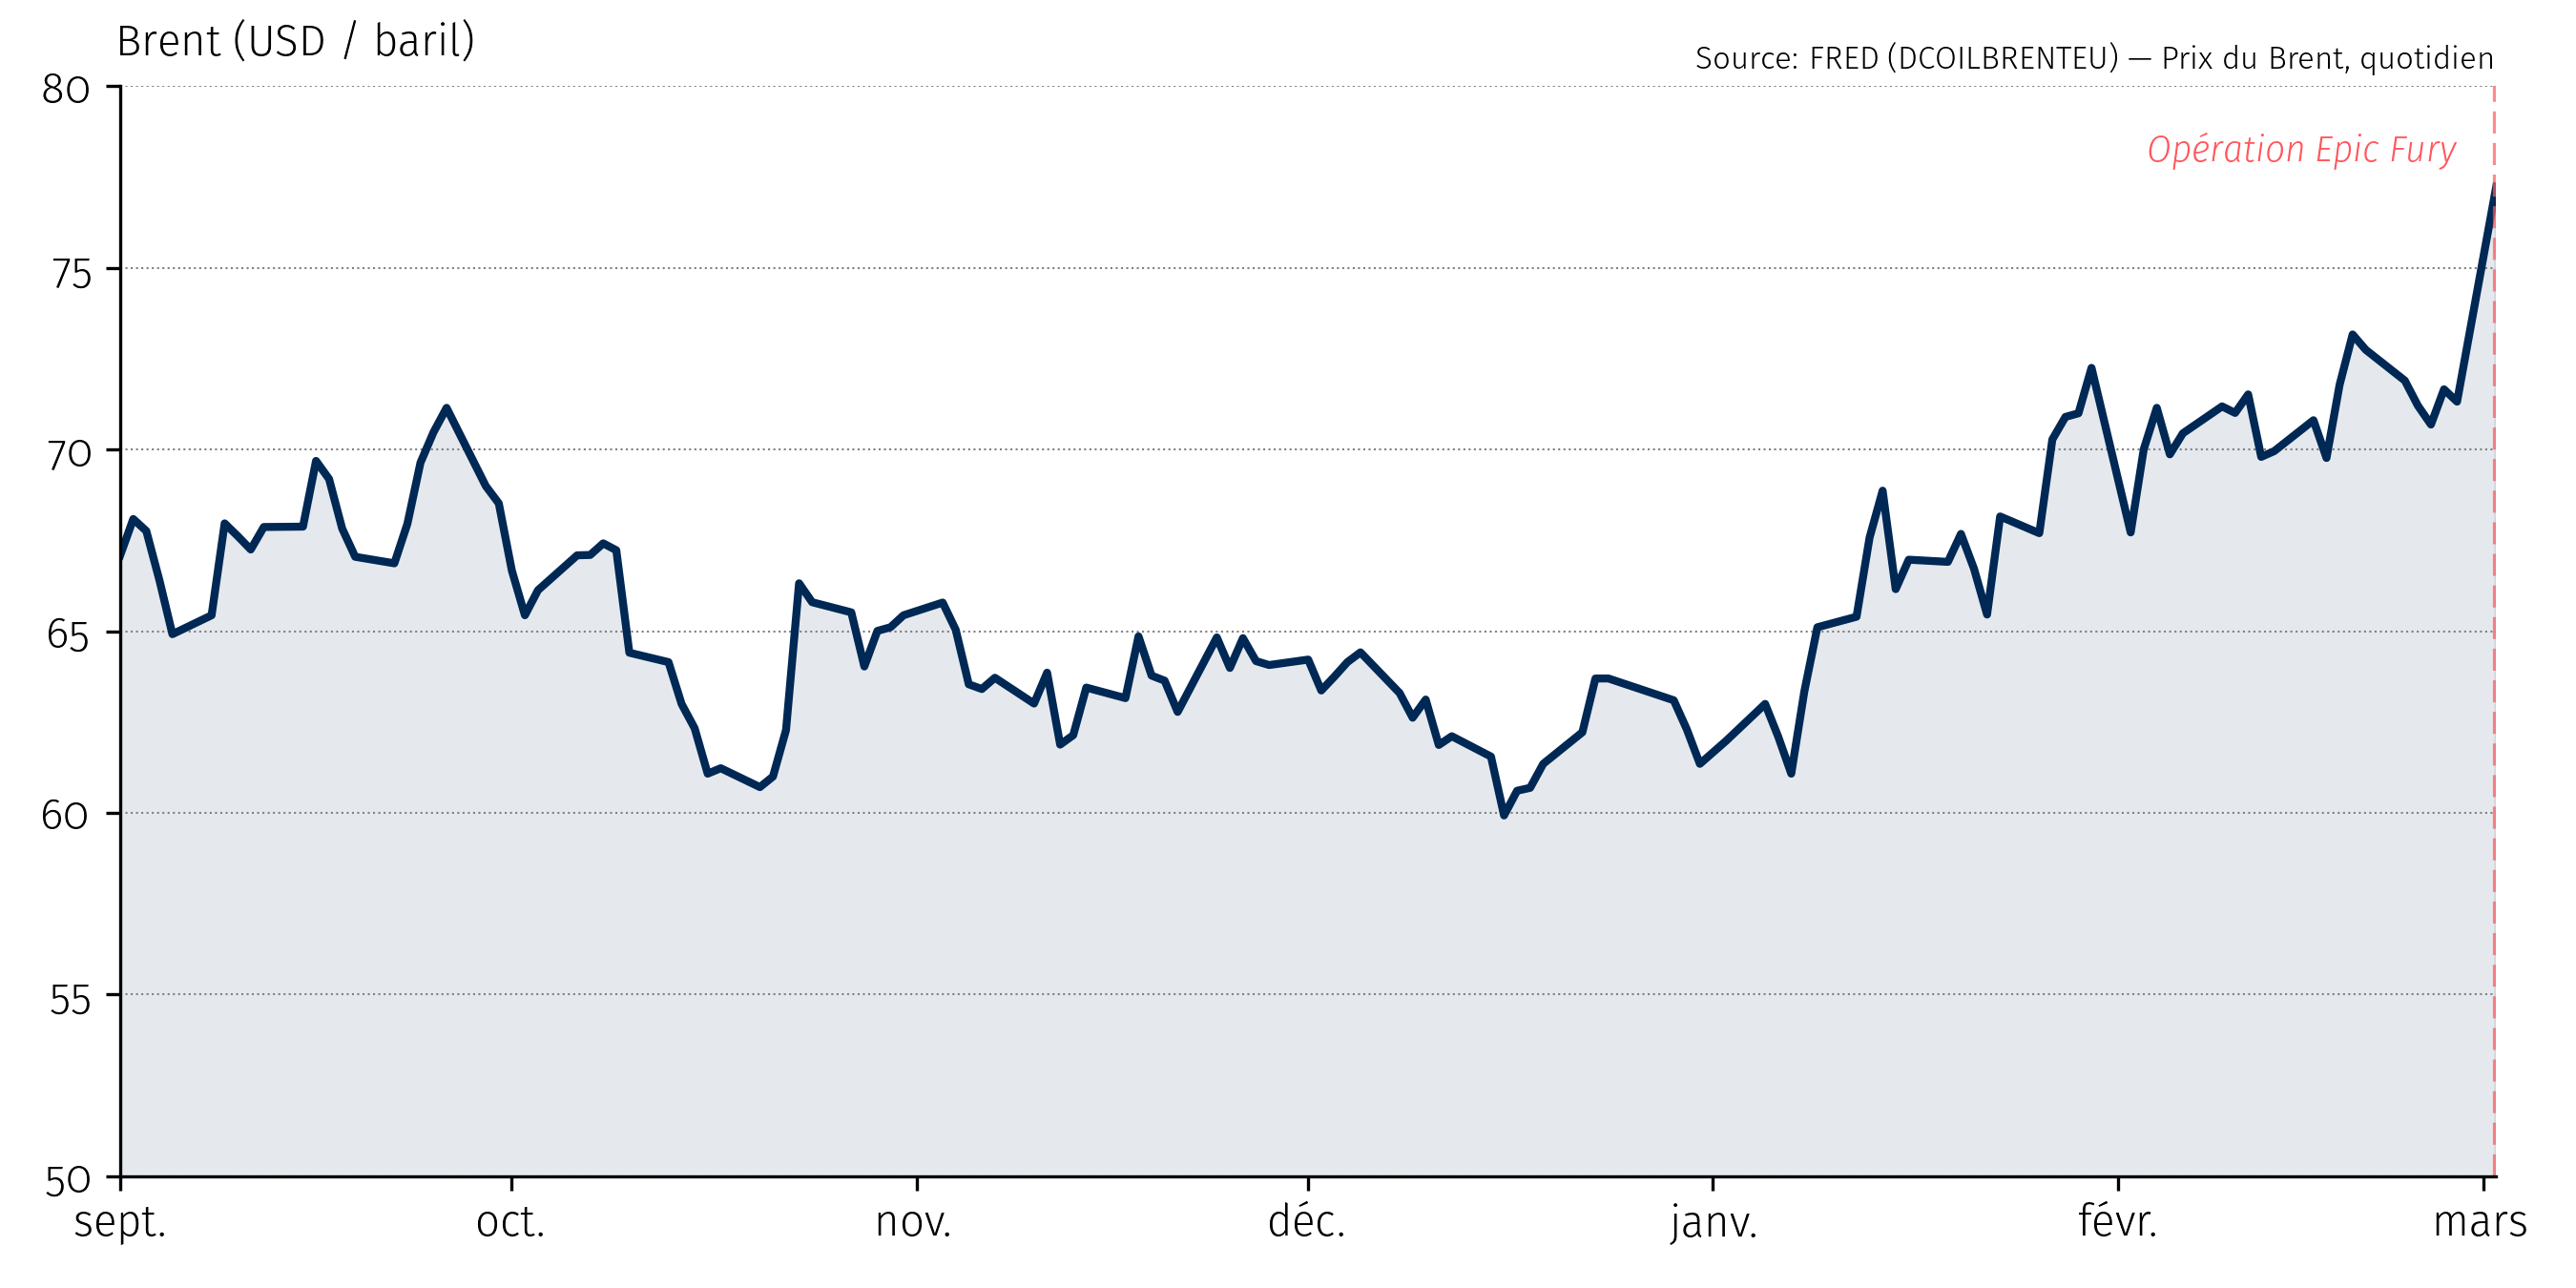
\includegraphics[width=0.95\textwidth, keepaspectratio]{oil_price_2026.png}
   \end{figure}
\end{frame}

\begin{frame}{2026 : AS domine $\to$ stagflation}
   \centering
   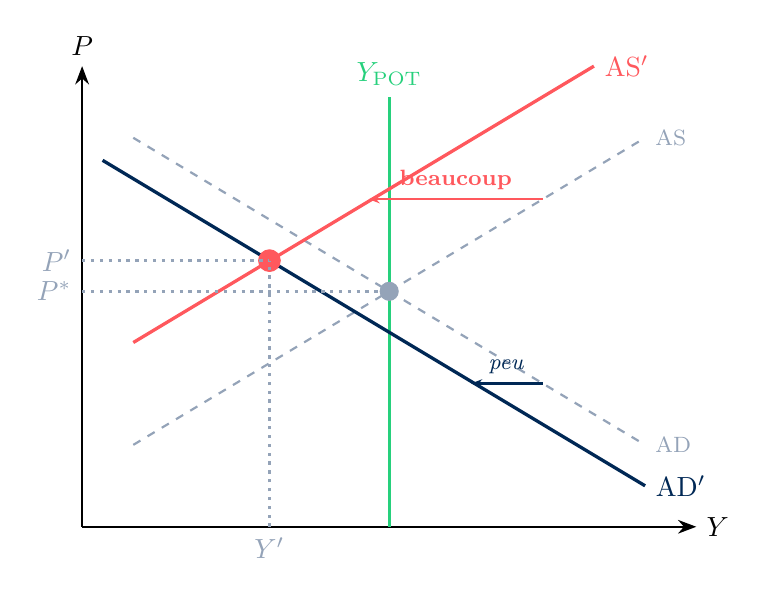
\begin{tikzpicture}[scale=1.3]
      % Axes
      \draw[-{Stealth}, thick] (0,0) -- (6,0) node[right] {$Y$};
      \draw[-{Stealth}, thick] (0,0) -- (0,4.5) node[above] {$P$};
      % Y_POT (vertical)
      \draw[HECgreen, very thick] (3.0,0) -- (3.0,4.2)
         node[above] {$Y_{\text{POT}}$};
      % AD original (dashed gray): y = -0.6x + 4.1
      \draw[HECgray, dashed, thick] (0.5,3.8) -- (5.5,0.8)
         node[right, font=\footnotesize] {AD};
      % AS original (dashed gray): y = 0.6x + 0.5
      \draw[HECgray, dashed, thick] (0.5,0.8) -- (5.5,3.8)
         node[right, font=\footnotesize] {AS};
      % AD' shifted slightly left: y = -0.6x + 3.7
      \draw[HECnavy, very thick] (0.2,3.58) -- (5.5,0.4)
         node[right] {AD$'$};
      % AS' shifted a lot left: y = 0.6x + 1.5
      \draw[HECcoral, very thick] (0.5,1.8) -- (5.0,4.5)
         node[right] {AS$'$};
      % Small AD shift arrow
      \draw[-{Stealth[length=4pt]}, HECnavy, thick] (4.5,1.4) -- (3.8,1.4);
      \node[font=\footnotesize, HECnavy, above] at (4.15,1.4) {\textit{peu}};
      % Large AS shift arrow
      \draw[-{Stealth[length=4pt]}, HECcoral, thick] (4.5,3.2) -- (2.8,3.2);
      \node[font=\footnotesize, HECcoral, above] at (3.65,3.2) {\textbf{beaucoup}};
      % Original equilibrium at (3.0, 2.3)
      \filldraw[HECgray] (3.0,2.3) circle (2.5pt);
      \draw[dotted, very thick, HECgray] (0,2.3) node[left] {$P^*$} -- (3.0,2.3);
      % New equilibrium: AD' ∩ AS' → x=1.83, y=2.60
      \filldraw[HECcoral] (1.83,2.60) circle (3pt);
      \draw[dotted, very thick, HECgray] (1.83,0) node[below] {$Y'$} -- (1.83,2.60);
      \draw[dotted, very thick, HECgray] (0,2.60) node[left] {$P'$} -- (1.83,2.60);
   \end{tikzpicture}
\end{frame}

\begin{frame}{Comment réagir face à une telle crise?}
   \centering
   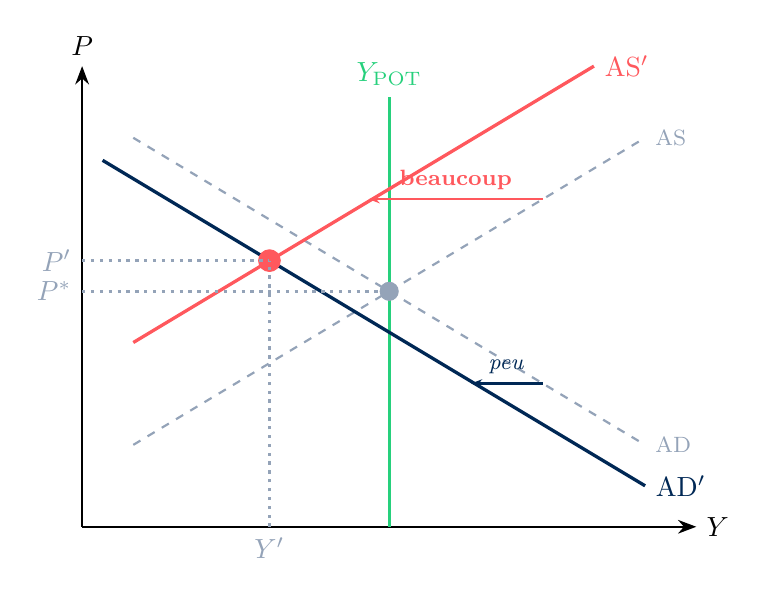
\begin{tikzpicture}[scale=1.3]
      % Axes
      \draw[-{Stealth}, thick] (0,0) -- (6,0) node[right] {$Y$};
      \draw[-{Stealth}, thick] (0,0) -- (0,4.5) node[above] {$P$};
      % Y_POT (vertical)
      \draw[HECgreen, very thick] (3.0,0) -- (3.0,4.2)
         node[above] {$Y_{\text{POT}}$};
      % AD original (dashed gray): y = -0.6x + 4.1
      \draw[HECgray, dashed, thick] (0.5,3.8) -- (5.5,0.8)
         node[right, font=\footnotesize] {AD};
      % AS original (dashed gray): y = 0.6x + 0.5
      \draw[HECgray, dashed, thick] (0.5,0.8) -- (5.5,3.8)
         node[right, font=\footnotesize] {AS};
      % AD' shifted slightly left: y = -0.6x + 3.7
      \draw[HECnavy, very thick] (0.2,3.58) -- (5.5,0.4)
         node[right] {AD$'$};
      % AS' shifted a lot left: y = 0.6x + 1.5
      \draw[HECcoral, very thick] (0.5,1.8) -- (5.0,4.5)
         node[right] {AS$'$};
      % Small AD shift arrow
      \draw[-{Stealth[length=4pt]}, HECnavy, thick] (4.5,1.4) -- (3.8,1.4);
      \node[font=\footnotesize, HECnavy, above] at (4.15,1.4) {\textit{peu}};
      % Large AS shift arrow
      \draw[-{Stealth[length=4pt]}, HECcoral, thick] (4.5,3.2) -- (2.8,3.2);
      \node[font=\footnotesize, HECcoral, above] at (3.65,3.2) {\textbf{beaucoup}};
      % Original equilibrium at (3.0, 2.3)
      \filldraw[HECgray] (3.0,2.3) circle (2.5pt);
      \draw[dotted, very thick, HECgray] (0,2.3) node[left] {$P^*$} -- (3.0,2.3);
      % New equilibrium: AD' ∩ AS' → x=1.83, y=2.60
      \filldraw[HECcoral] (1.83,2.60) circle (3pt);
      \draw[dotted, very thick, HECgray] (1.83,0) node[below] {$Y'$} -- (1.83,2.60);
      \draw[dotted, very thick, HECgray] (0,2.60) node[left] {$P'$} -- (1.83,2.60);
   \end{tikzpicture}
\end{frame}

\begin{frame}{Que faire face à une récession?}
   \vspace{0.3cm}
   \textbf{Analyse en quatre étapes :}
   \vspace{0.3cm}
   \begin{enumerate}
      \setlength\itemsep{0.3cm}
      \item {\color{gray!50}Étincelle --- ce qui déclenche la récession}
      \item {\color{gray!50}Transmission --- comment le choc se propage}
      \item {\color{gray!50}Carburant --- ce qui amplifie la transmission}
      \item \textbf{\textcolor{HECnavy}{Pare-feu --- réponse politique pour limiter les dégâts}}
   \end{enumerate}
   \vspace{0.3cm}
   \begin{keyinsight}
      L'économie peut se corriger seule, mais \textbf{attendre coûte cher} (chômage, faillites). C'est le fondement de la politique contracyclique $\to$ \textbf{Séance 5}.
   \end{keyinsight}
\end{frame}

% ============================================================================

\begin{frame}{}
   \centering
   \vspace{1.5cm}
   {\Large\textbf{Qu'est-ce que vous retenez de cette séance?}}
\end{frame}

% ============================================================================
\sectionframe{Et pour la suite?}
% ============================================================================

\begin{frame}{Thèmes et séances à venir}
   \renewcommand{\arraystretch}{1.5}
   \centering
   \small
   \begin{tabularx}{\textwidth}{>{\bfseries}X l}
      \toprule
      \textbf{Thème} & \textbf{Séance} \\
      \midrule
      Pourquoi/comment combattre les récessions? & S5 : Pol.\ mon.\ et budgétaire \\
      Quel avenir pour la mondialisation? & S6 : Commerce international \\
      \bottomrule
   \end{tabularx}
\end{frame}

\end{document}
